% !TeX program = pdflatex
% !TeX encoding = UTF-8

%==============================
% Splatone Preprint (Skeleton)
%==============================

\documentclass[11pt,a4paper]{jlreq}

%--------- Packages ----------
\usepackage[T1]{fontenc}
\usepackage[utf8]{inputenc}
\usepackage{lmodern}
\usepackage{amsmath,amssymb,amsthm}
\usepackage[dvipdfmx]{graphicx}
\usepackage{tikz}
\usetikzlibrary{arrows.meta, positioning}
\usepackage{authblk}
\usepackage{url}
\usepackage{hyperref}
\usepackage{geometry}
\geometry{margin=25mm}
\usepackage{listings}
\usepackage{xcolor} % 色を使う場合
\usepackage{svg}

\svgpath{{figures/}}
%\svgsetup{inkscapelatex=true, inkscapepath={C:/Program Files/Inkscape/bin/}}

\lstdefinestyle{commandline}{
  basicstyle=\ttfamily\small,
  backgroundcolor=\color{black!5},
  frame=single,
  columns=fullflexible,
  keepspaces=true,
  escapeinside={}
}

\lstnewenvironment{commandline}[1][]{
  \lstset{style=commandline,#1}
}{}

\lstdefinestyle{commandstdout}{
  basicstyle=\ttfamily\small\color{white},
  backgroundcolor=\color{darkgray},
  frame=single,
  columns=fullflexible,
  keepspaces=true,
  escapeinside={(*@}{@*)}
}

\lstnewenvironment{commandstdout}[1][]{
  \lstset{style=commandstdout,#1}
}{}

%--------- Meta data ----------
\title{Splatone crawler: ジオソーシャルデータの収集・可視化のための汎用ツール}

% TODO: 著者情報を埋めてください
\author[1]{横山昌平}
\affil[1]{東京都立大学, 東京都日野市旭が丘6-6}

\date{\today}

%--------- Document ----------
\begin{document}

\maketitle

\begin{abstract}
  % このツール Splatone の概要を1段落で記述して。
  位置情報付き画像コレクションは,観光行動や都市空間の理解に有用な情報源として注目されているが,その空間的・時間的な不均一性や膨大な量により,単純な地図表示では全体の傾向把握が困難である.
  本研究では,位置情報付き画像の色彩情報と位置情報を統合的に扱う可視化ツールSplatone Crawlerを提案する.
  Splatone Crawlerは,知覚的距離に基づいた自動カラーパレット生成と,地理空間上のVoronoi分割,クラスタリング,グリッド集計など複数の可視化手法を組み合わせることで,ジオタグ位置分布だけでなく,カテゴリごとの空間配置を直感的に把握できることを目指す.
  また,ツール本体はProviderとVisualizerを差し替え可能な拡張機構を備えており,新たなデータソースや可視化手法を容易に追加できる点も特徴である.
  提案手法の実装系は GitHub および NPM にて公開されており,誰でも利用可能である.
  本論文ではそのシステム構成、利用方法、および利用事例を示す.
\end{abstract}

\section{はじめに}
近年,位置情報付きソーシャルデータを分析・活用するための基盤は整いつつあるものの,(1) カテゴリ(キーワード集合)間の空間的差異を同一フレームで比較しづらい,(2) 可視化手法ごとの前処理(グリッド化,クラスタリング等)が個別実装になり再利用性が低い,(3) 高視認性彩色と地理的構造(密度・境界・混在度)を統合した視覚表現が不足している,といった課題が残されている.特に複数キーワードを束ねたカテゴリ単位での比較は,単純な点描画だけでは分布の偏り・重なり・局所的特徴を解釈しにくく,分析者がズーム・パンを繰り返す探索的操作に依存しがちである.


本研究で提案するSplatone Crawlerは,これらの課題に対処するため,クローリングから色特徴抽出・空間集約・複数可視化への受け渡しを一貫パイプライン化し,かつProvider/Visualizer拡張を前提とした枠組みを提供する.本ツールの主な特徴と貢献を以下に整理する.
\begin{itemize}
  \item ワーカープロセスを介した非同期クローリングによる大規模データ収集の効率化
  \item GeoJSON形式によるデータモデルの統一化と可視化手法間の連携容易化
  \item カテゴリ(複数キーワード集合)概念の導入による柔軟な OR 検索とカテゴリ別比較
  \item 知覚距離に基づく自動パレット生成の統合(色の一貫した割当)
  \item 六角グリッド・Voronoi・密度(KDE)・クラスタ(DBSCAN)・割合円グラフ等,異なる空間表現の並列提供
  \item 可視化/取得対象(Provider, Visualizer)のモジュール化による第三者拡張性
  \item コマンドライン起動とブラウザ UI の即時連携による試行錯誤的探索支援
\end{itemize}

これにより,単一手法では捉えにくかった「カテゴリ間の空間的入れ替わり」「局所的優勢の分布可視化」「高密度点群区域の内部構造」などを多面的に観察できる.以降では関連研究を概観した後(第\ref{sec:related}章),データモデルと全体構成(第\ref{sec:overview}章),色彩情報を活用する可視化手法群(第\ref{sec:colorviz}章),拡張を可能にする実装上の工夫(第\ref{sec:implementation}章),具体的利用事例(第\ref{sec:usecases}章),最後に考察と今後の課題(第\ref{sec:discussion},\ref{sec:conclusion}章)を述べる.

近年,Flickr をはじめとする写真共有サービスや,SNS 上で投稿される写真には位置情報が付与されることが一般的になり,大規模な位置情報付き画像コレクションが容易に取得できるようになっている.
これらのデータは,人々の移動や観光行動,都市空間の使われ方など,従来の調査では把握が難しかった現象を分析するための有力な情報源として注目されている.
一方で,位置情報付き画像は空間的・時間的に不均一かつ量が膨大であり,単純に地図上にマーカとして表示するだけでは,全体の傾向や特徴的なパターンを把握することが難しい.

こうした課題に対し,地理空間上での分布や時空間パターンを可視化・解析するための手法がこれまでに多数提案されている.
例えば,K{\'a}d{\'a}r ら\cite{kadar2013wheredotouristsgo} は観光客によって撮影された位置情報付き写真の空間分布を解析し,観光地内での人気エリアや動線を明らかにしている.
また,Kisilevich ら\cite{kisilevich2010eventbased} は Flickr および Panoramio の画像を用いてイベントに関連する人々の活動パターンを抽出し,クラスタリング結果を地図上に可視化している.
これらの研究は,位置情報付き写真が観光や都市解析に有用であることを示しているが,可視化の多くは密度マップやクラスタ境界の表示に留まっており,色やカテゴリ情報を手がかりにした多面的な可視化環境は必ずしも十分ではない.

本研究では,位置情報付き画像コレクションの色彩情報と位置情報を統合的に扱う可視化ツールSplatone Crawlerを提案する.
Splatone Crawlerは,知覚的距離に基づいた自動カラーパレット生成と,地理空間上のVoronoi分割,クラスタリング,グリッド集計など複数の可視化手法を組み合わせることで,ジオタグ位置分布だけでなく,カテゴリごとの空間配置を直感的に把握できることを目指す.
また,ツール本体はProvider/Visualizerを差し替え可能な拡張機構を備えており,新たなデータソースや可視化手法を容易に追加できる点も特徴である.

なお,Splatone CrawlerはGitHub \footnote{https://github.com/YokoyamaLab/Splatone}およびNPM \footnote{https://www.npmjs.com/package/splatone}にて公開されており,誰でも使う事が可能となっている.

本論文の構成は次のとおりである.
第\ref{sec:related}章では,位置情報付き写真の可視化および分析に関する関連研究を概観する.
第\ref{sec:overview}章では,Splatone Crawlerのデータモデルとシステム構成を説明する.
第\ref{sec:colorviz}章では,本研究で実装したカラーベースの可視化手法と,各Visualizerの役割について述べる.
第\ref{sec:implementation}章では,実装上の工夫や拡張機構について説明し,第\ref{sec:usecases}章で利用事例を示す.
最後に,第\ref{sec:discussion}章および第\ref{sec:conclusion}章で考察と結論を述べる.

\section{関連研究}
\label{sec:related}
位置情報付き写真を利用した可視化および分析に関する研究は,観光行動の解析,都市空間の理解,イベント検出など多様な文脈で行われている.
K{\'a}d{\'a}r ら\cite{kadar2013wheredotouristsgo} は,Flickr などから収集した位置情報付き写真を用いて,観光客がどこへ行くのかを可視化し,観光地における人気スポットや移動パターンを明らかにした.
彼らは写真の空間分布を地図上に表示しつつ,滞在時間や移動経路を解析することで,観光行動の偏りやホットスポットを定量的に評価している.

Kisilevich ら\cite{kisilevich2010eventbased} は,Flickr および Panoramio の位置情報付き画像コレクションに対しクラスタリングを適用し,イベントに関連する人々の活動パターンを抽出する手法を提案した.
クラスタ境界を密度等値線に基づくポリゴンとして可視化することで,特定イベントに紐づく空間的な広がりや集積度を地図上で把握できる.
Hu ら\cite{hu2015extractingAOI} は,複数都市の位置情報付き写真から,都市内の関心領域(Area of Interest)を抽出し,土地利用との関係を分析している.
Lee ら\cite{lee2014exploration} は,データマイニング手法を用いて位置情報付き写真のクラスタリングやパターン抽出を行い,地理空間的な利用パターンの理解に貢献している.

これらの研究はいずれも,位置情報付き写真が観光・都市解析の有効な情報源であることを示すとともに,空間分布やクラスタ構造の可視化に主眼を置いている.
一方で,写真に含まれる色やカテゴリといった視覚的特徴を,地理空間上の表現と密接に結びつけて対話的に探索できる汎用ツールはまだ限られている.
本研究のSplatone Crawlerは,色彩情報と空間情報を同時に扱う複数のVisualizerを統合的に提供する点で,既存研究を補完する可視化環境を目指している.

本研究で採用するボロノイ分割は,空間点集合から局所的勢力圏(最近領域)を定義し密度勾配や遷移境界を可視化する代表的手法であり,基礎理論と応用を体系化した Okabe らの著作\cite{okabe2000spatial}が広く参照されている.

格子集約系では等間隔正方格子より方向バイアスが少なく近傍関係が均質な六角ビニング\cite{carr1987hexbin}が大量点群の密度とカテゴリ比率表示に有効とされる.連続的密度場の推定にはカーネル密度推定(KDE)が用いられ,帯域幅選択やスムージングの統計的基盤は Silverman\cite{silverman1986density} により整理された.
クラスタ的構造の抽出と境界可視化にはノイズ耐性を持つ密度ベース手法 DBSCAN\cite{ester1996dbscan} が頻用され,観光・都市写真分布の局所集積検出に適用されている.

さらに点群のスケール非依存な空間パターン評価には Ripley の K 関数\cite{ripley1976second} が用いられ,K 曲線とランダム基準の差異を併置することで過密・過疎領域の多尺度的特徴を補助的に説明する可視化が提案されている.これら手法を組み合わせることで,単一表示では捉えにくい境界・密度・カテゴリ混在度を多面的に把握可能となる.

本論文では,それらこれまでの可視化手法を統合・複合的に利用できる他,Provider/Visualizerアーキテクチャにより第三者による機能拡張も容易である.著者自身もHexGridと円グラフを組み合わせて複数のカテゴリに跨ったヒートマップを同一地図上に可視化するMajority Hexを提供している.
\section{システムの概要}
\label{sec:overview}

\subsection{用語定義}

\subsubsection{Splatone Crawler}

提案するシステムであり,SNSから複数のキーワードでジオタグ付きデータを検索し,キーワード毎の分布の違いを分析するために効果的な可視化を行う.
柔軟なプラグインアーキテクチャを採用しており,ProviderとVisualizerという二系統の拡張機能を持つ.
Providerはデータを集める対象となるサービス毎に構成し,現在のバージョンではFlickrのみに対応しているが,アーキテクチャはオープンである.
Visualizerはクローリングしたジオタグ付きデータを地図上に描画するための機能であり,これもサードパーティによる追加が可能である.
これらの詳細については後述するが,単純な可視化のみならず,ヒートマップ,Voronoi図,DBSCANクラスタリング,HexGrid集約など多様な可視化手法を実装している.

\subsubsection{HexGrid}

HexGridとは六角形の格子であり,地理空間上での集約処理に用いられる.
六角形は正方形に比べて隣接セルが6つと多く,方向バイアスが少ないため,地理空間上での集約処理に適している.
Splatone Crawlerでは,HexGridを用いてジオタグ付きデータの集約処理を行い,各セル内でのカテゴリ割合や密度を計算する事ができる.
HexGridはユーザが指定したセルサイズに基づいて、ユーザが指定したBoundary(矩形または多角形)
を包含するように生成される.
基本的にはこのHexGridがクローリングにおけるクエリ空間分割に利用される他、可視化における集約単位として用いられる。
ただし、可視化においては、必ずしもGrid-basedの手法を用いる必要はなく、集約なしでの全量可視化やDBSCANなどの密度ベースの可視化を行う事も可能である。

\subsubsection{キーワードとカテゴリ}

キーワードはソーシャルデータの検索に用いる単語の事である.例えばFlickrから森林の写真と海岸の写真の撮影位置を可視化したい場合,森林や海岸をキーワードとして指定すればよい.

ただし検索したい対象は一語のみで得られるとは限らない.例えば森林についてもう少し幅広く写真を集める場合,ジャングルやタイガ等のキーワードでも検索し,結果を一緒に扱いたい,すなわちOR検索をしたい場合が多い.
本システムでは,カテゴリという概念を用いてそれを実現している.
カテゴリとは複数のキーワードを束ねる概念であり,ラベルを付ける事ができる.
森林,ジャングル,タイガというキーワード群に対して,例えば緑地というラベルを付ける等の利用法を想定している.
この緑地という文字自体は検索には用いられず,森林,ジャングル,タイガという複数のキーワードを束ねる概念として可視化ページの凡例等で用いられる.

なおラベルは必須ではなく,キーワード群のみでカテゴリを定義する事も可能である.その場合は最初のキーワードがラベルとして用いられる.

\subsubsection{Provider}

Splatone Crawlerはジオソーシャルデータに特化したクローラーであるが,集める対象のサービスは限定しておらず,Providerと呼ぶプラグイン機構により,収集対象サービスのAPIをラップする事で,複数のジオソーシャルデータサービスに対応できるようになっている.
現在のバージョンではFlickrのみに対応しているが,アーキテクチャはオープンであり,第三者が新たなProviderを追加する事も可能である.

Providerの動作は非同期であり,ワーカープロセスを用いて並列にクローリングを行う事ができる.並列度はコマンドライン引数で指定可能であり,これにより大規模なジオソーシャルデータの収集を効率的に行う事ができる.
多くのサービスでは,APIの利用制限が設けられており,一定時間内に実行できるリクエスト数が制限されている.Providerはこの制限に対応するため,リクエストの最低実行間隔を指定する事ができ,これにより,APIの利用制限を超えないように設計されている.
\subsubsection{Visualizer}

Visualizerは可視化手法をパッケージ化したものであり,これもプラグイン機構により第三者が任意の可視化手法を追加する事が可能である.
拡張アーキテクチャにより,Visualizerはメインルーチンを侵食する事なく,サーバ側処理とブラウザ側処理を記述する事ができ,目的に応じて処理を配置する事ができる.
現在は以下の可視化手法を実装している.
\begin{itemize}
    \item Bulky: クロールした全てのジオタグを小さな点で描画する
    \item Marker Cluster: 密集しているジオタグをクラスタリングしてまとめて表示する
    \item Pie Charts: HexGridに基づく可視化.セル中心にカテゴリ割合のPie Chartを描画し,カテゴリごとに半径を可変
    \item Majority Hex: HexGridの各セルをセル内で最頻出するカテゴリの色で彩色
    \item Heat: KDEによるヒートマップ
    \item Pie Charts: 円グラフグリッド
    \item Voronoi: HexGrid単位で集約したジオタグからVoronoiセルを生成し,各Hexのポリゴンでクリップして表示
    \item DBSCAN: ジオタグをDBSCANクラスタリングし,KDEベースの等値線で近似した境界ポリゴン(不足時のみ凸包)を表示
\end{itemize}

\subsection{Splatone Crawler CLI}
% この説ではCLIの仕様について述べる
Splatone CrawlerはJavaScriptにより実装されたツールであり,Node.jsの環境で動作する.
またNode Package Execute (npx)での起動に対応しているため,Node.jsの環境さえ準備すれば,インストール等の環境構築は一切不要である.
Splatone CrawlerのUsageを表示するコマンドは以下の通りである.

\begin{commandline}
npx -y -p splatone@latest crawler --help
\end{commandline}


Command Line Interface(CLI)で起動するとWebサーバを立ち上げた後,Webブラウザを自ら立ち上げて,サーバ・クライアント型のシステムとして動作する.
サーバ側ではSNSからのクローリングや可視化のための前処理を行い,地図上での可視化はWebブラウザ側で行う.また,npxによる起動に対応しているため,Node.jsの環境さえ準備すれば,インストール等の環境構築は一切不要である.

さらに,前述したProviderとVisualizerという二系統のプラグイン機能を持ち,複数のジオソーシャルデータに対して,複数の可視化・分析を行う事ができる.
Providerはデータを集める対象となるサービス毎に構成し,Visualizerは描画方法毎に構成する.これらのアーキテクチャはオープンであり,第三者が新たなProviderやVisualizerを追加する事が可能である.

例として以下に最小構成のコマンドを記す.このコマンドでは写真共有サイトFlickrから撮影位置の緯度経度が付与された写真をクローリングし,地図上にマップする.なお,\texttt{--p-flickr-APIKEY}はFlickrのAPIキーであり,各自で取得したものに置き換える必要がある.

\begin{commandline}
npx -y -p splatone@latest crawler -p flickr -k "canal,river|street,alley|bridge"\
--vis-bulky --p-flickr-APIKEY="aaaaaaaaaaaaaaaaaaaaaaaaaaaaaaaaa"
\end{commandline}

コマンドを実行すると,Webブラウザが立ち上がり地図が表示される.
地図はマウスでスクロールでき,拡大・縮小も可能である.
ここで任意の場所を矩形ツールで指定しStart Crawlingボタンを押下する事で,クローリングが開始される.しばらくたつと当該領域の指定したキーワードを持つジオタグ付き写真の収集が完了し,地図上に表示される.

\begin{figure}[h]
  \centering
  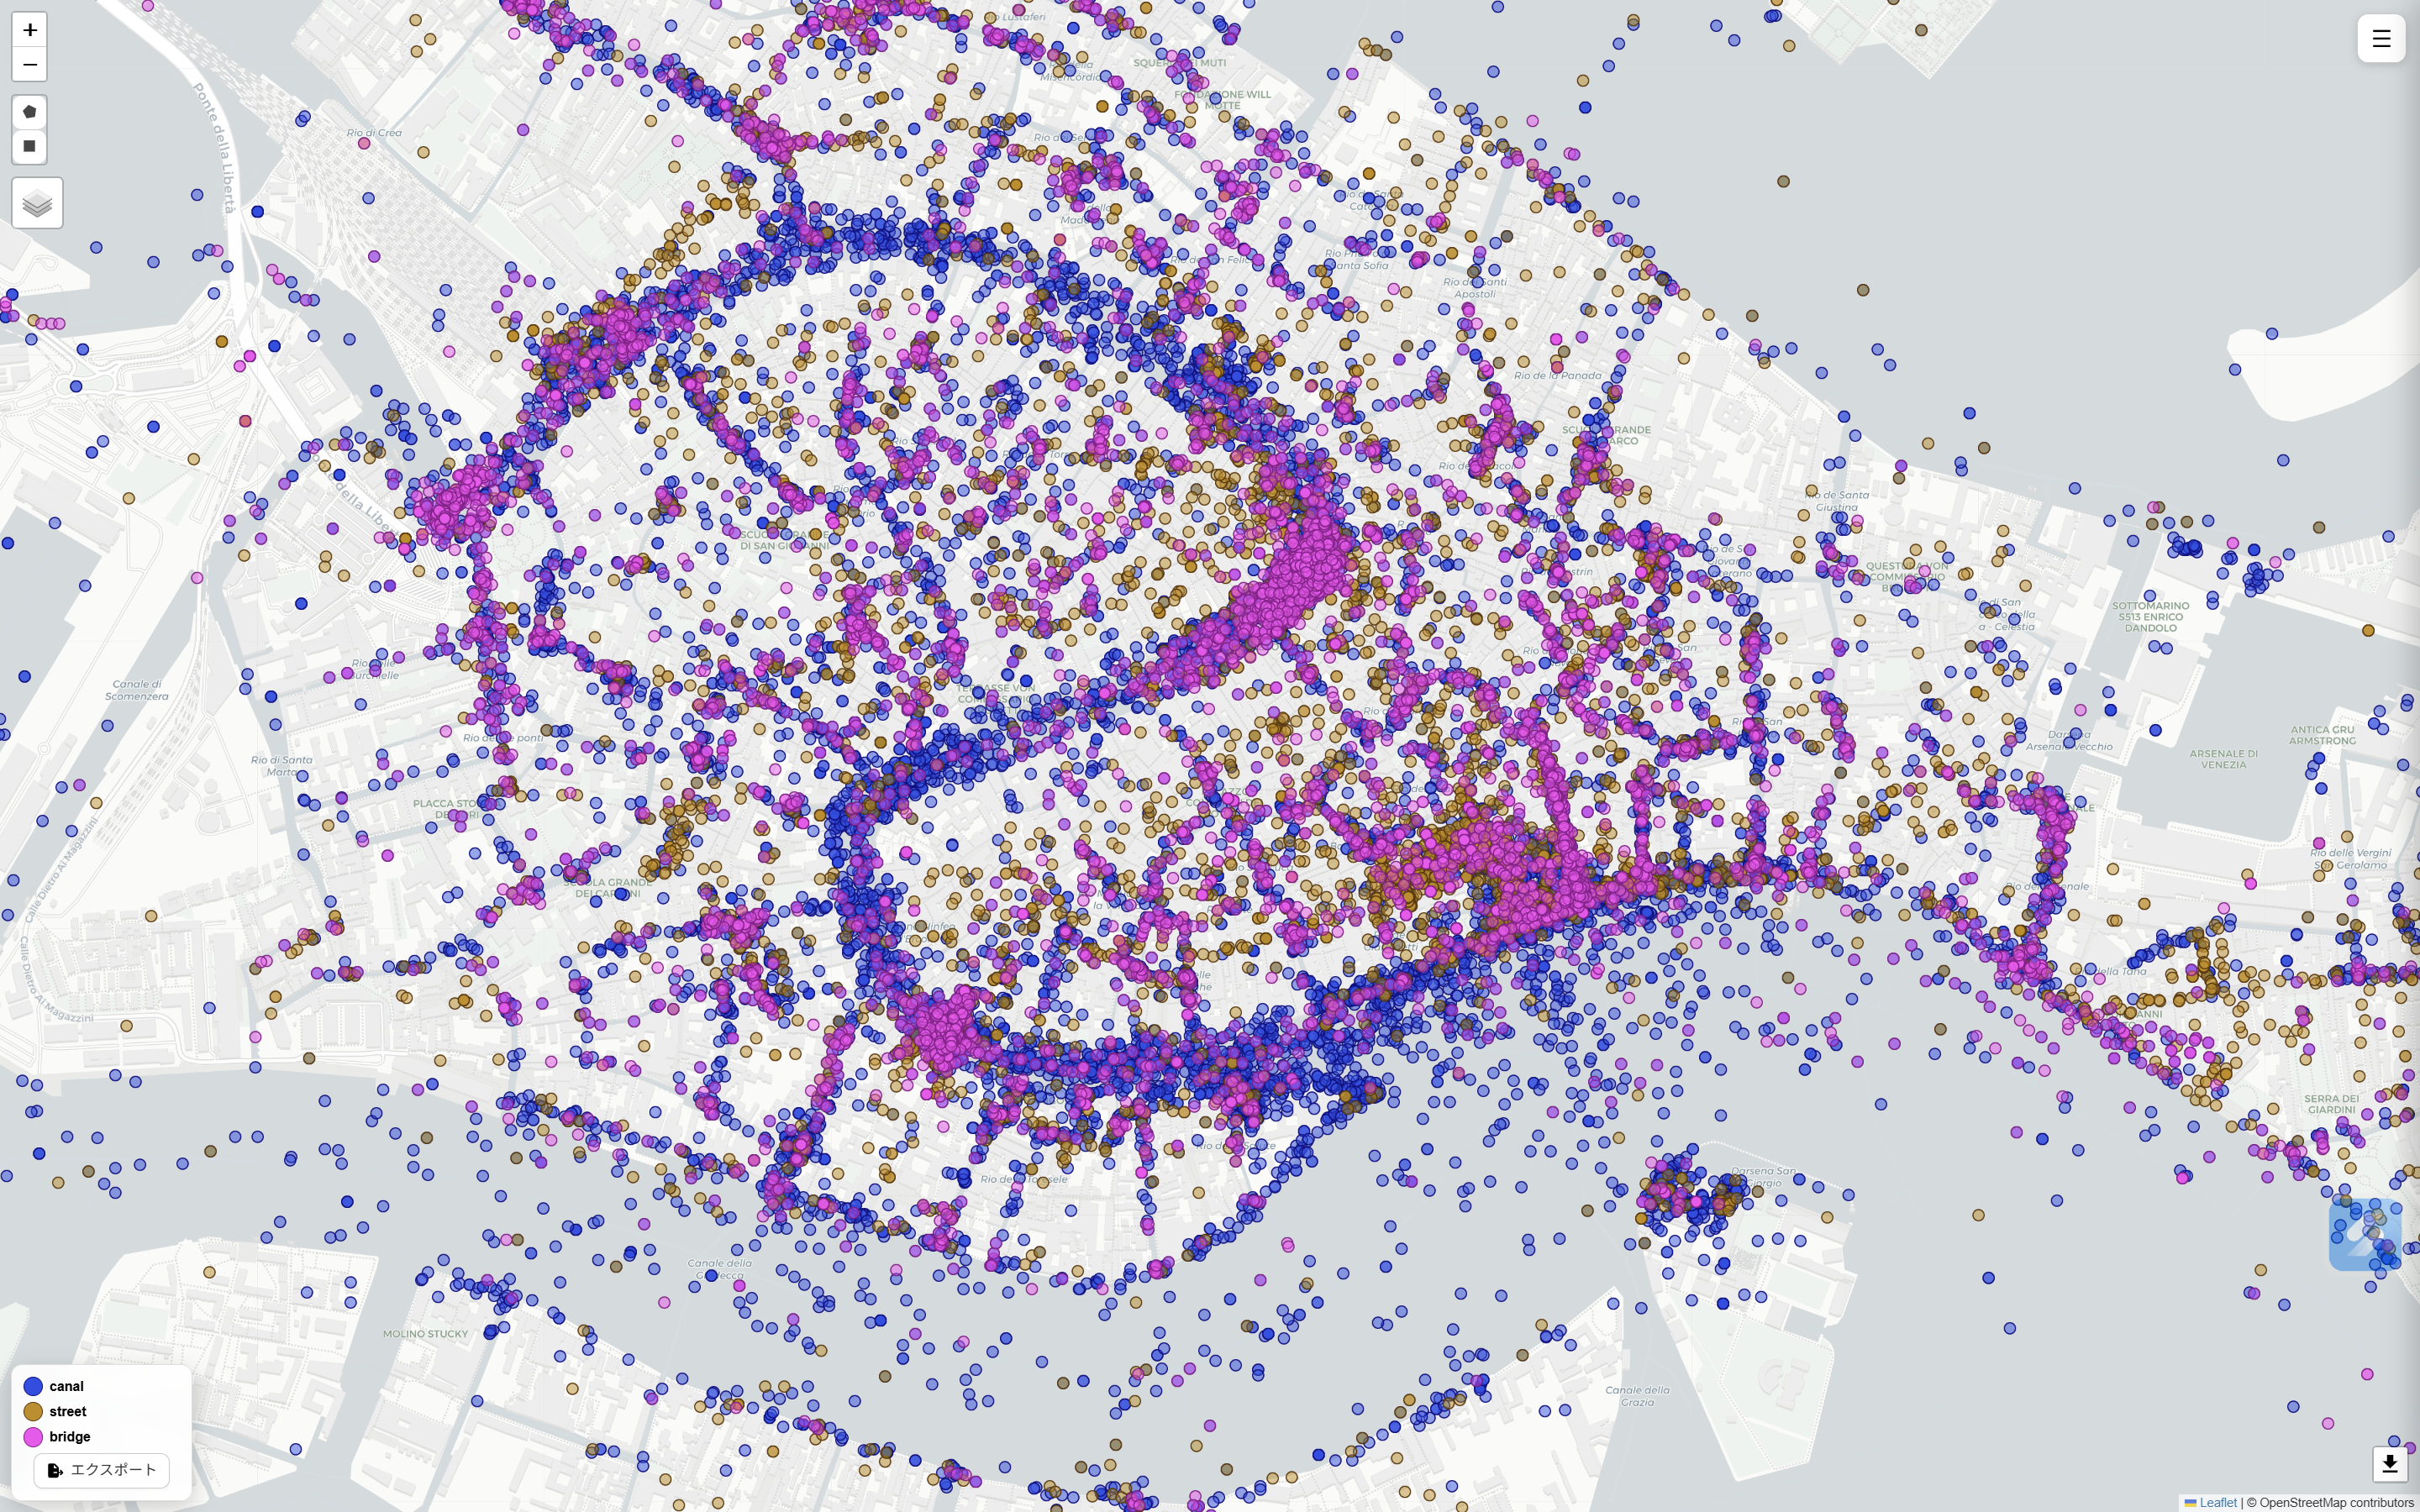
\includegraphics[width=0.5\textwidth]{figures/result_venezia_bulky.png}
  \caption{ベネチアの結果例(bulky版)}
  \label{fig:venezia_bulky}
\end{figure}

\subsection{Data Model}
% 画像, メタデータ (位置, タグなど) の扱い

\subsubsection{Splatone Unified Feature Schema (SUFS)}
Providerごとの応答形式を吸収し,Visualizerが一貫した前処理を受け取れるように設計した内部データモデルを\textbf{Splatone Unified Feature Schema(SUFS)}と呼ぶ.SUFSはGeoJSONを基底フォーマットとしつつ,カテゴリ情報,色パレット,進捗統計,補助的なジオメトリ(例:HexGridや三角分割)を束ねた複合バンドルで構成される.そして外部サービス毎に異なるAPIレスポンスはProviderがSUFS互換のFeatureCollectionへ正規化する.

Splatone Crawlerの対象とするデータは位置情報付きドキュメント(例えばジオタグ付き画像)であるため,一つのドキュメントはPointジオメトリを持つFeatureとして表現される.クローリングされた複数ドキュメントの集合は点群を内包するFeatureCollectionとしてまとめられ,Visualizer側へ受け渡される.Featureはジオメトリだけでなくプロパティを保持する事ができ,Visualizer側での描画に必要なメタデータや,さらなる分析に必要な補助情報を格納できる.例えばFlickrのジオタグ付き写真の場合はプロパティに写真のIDや撮影者ID,撮影時刻,タグ,画像のURLなどを含めることができる.

Visualizer側はProviderから得られたSUFSのFeatureCollectionに対して可視化処理を行い,結果をFeatureCollectionとして返す.例えばVoronoi図を描画する場合,点群からVoronoiセルを計算し,各セルをポリゴンジオメトリとして持つFeatureCollectionを生成する.これを地図上で表示する事で,Voronoi図を可視化できる.一方で点群をそのまま地図上に表示するBulky可視化の場合,Providerから受け取ったFeatureCollectionをそのまま地図に描画する.どちらのケースも,GeoJSONを基底に持つSUFSを介してデータが受け渡されるため,VisualizerはProviderの実装に依存せず,ブラウザ上ではSUFSと補助メタデータを受け取るだけで描画を開始できる.これにより,新たなProviderを実装する場合でもSUFSへのマッピングさえ行えば既存のVisualizer群がそのまま機能し,逆にVisualizerを追加する場合もSUFSを入力として設計すればProvider追加の有無に依存しない拡張が可能となる.

一点補足をすると,Visualizerは複数指定する事ができる.例えばVoronoi図とDBSCANクラスタリングを同時に指定した場合,Providerから受け取ったSUFSをそれぞれのVisualizerが独立に処理し,Voronoi図用のFeatureCollectionとDBSCANクラスタリング用のFeatureCollectionを生成する.これらは地図上で別々のレイヤとして描画される.それにより,同一のジオタグ付き画像データに対して複数の可視化手法を適用し,ユーザが目的に応じて視点を切り替えながら探索できるようにしている.

データモデルについてまとめる.SUFSはProviderとVisualizer間のデータ受け渡しだけでなく,Visualizer内のサーバ・クライアント間でのデータ受け渡しにも用いられる.前者はProviderが生成したFeatureCollectionをVisualizerが受け取る場合であり,後者はVisualizerのサーバ側処理が生成したFeatureCollectionをブラウザ側処理が受け取る場合である.混同を避けるために,以降ではProvider-Visualizer間の受け渡しを\texttt{SUFS/Naked},Visualizer内のサーバ・クライアント間の受け渡しを\texttt{SUFS/Compiled}と呼ぶ事にする.

\subsection{Architecture}

\begin{figure}[h]
  \centering
  \includesvg[width=1\textwidth,inkscapelatex=false]{overall}
  \caption{Splatone Crawler の全体構成}
  \label{fig:architecture}
\end{figure}

Splatone Crawlerの全体構成を図~\ref{fig:architecture}に示す.
本ツールは大きく,(1)画像およびメタデータを取得するProvider層,(2)取得データに対して前処理やカラーパレット生成・空間集計を行うコアライブラリ層,(3)結果をWeb UIを通じて提示するVisualizer層から構成される.

Provider層では,各ジオソーシャルデータサービスのAPIをラップし,クエリに基づいて位置情報付き画像とメタデータを収集する.

コアライブラリ層では,コマンドライン引数で与えられるクエリの解釈と,HexGridを用いたクエリ分割とワーカープロセスによる非同期クローリングを組み合わせて大規模データの収集を効率化するとともに,クエリ進捗管理およびWeb UIへの進捗通知を担当する.

Visualizer層では,コアライブラリ層から受け取った位置情報付き画像データを,ユーザが指定した複数の可視化手法に基づいて地図上に描画する.

\section{Color-based Visualization}
\label{sec:colorviz}
\subsection{Palette Generation}
Splatone Crawlerでは,位置情報付き画像集合に対して色の要約表現を与えるために,カラーパレットを自動生成する.

自動生成にはchroma.js \footnote{\url{https://gka.github.io/chroma.js/}} を用いており、具体的にはCIELAB色空間における色の分布をK-meansクラスタリングにより要約し,代表色を抽出する事で、カテゴリ数に応じて知覚的に均等に分布したカラーパレットを生成する.

ただしカテゴリに適した色をユーザが手動で指定する事も可能である.例えば海に関するカテゴリには青系統の色を,森林に関するカテゴリには緑系統の色を割り当てる等の利用法を想定している.
Splatone Crawlerではカラーパレットの手動指定を補助するコマンドを持っており、例えば4色に塗分けたい場合、以下のコマンドを実行する事で,4色の自動生成パレットを5セット取得できる.

\begin{commandline}
npx -y -p splatone@latest colors 4 5
\end{commandline}

このコマンドを実行すると,以下のような出力が得られる.

\begin{commandstdout}
(*@\textcolor[HTML]{FC00FF}{\#FC00FF}@*),(*@\textcolor[HTML]{41FFB2}{\#41FFB2}@*),(*@\textcolor[HTML]{882600}{\#882600}@*),(*@\textcolor[HTML]{329FFF}{\#329FFF}@*)
(*@\textcolor[HTML]{000AF3}{\#000AF3}@*),(*@\textcolor[HTML]{85C500}{\#85C500}@*),(*@\textcolor[HTML]{FF1DA7}{\#FF1DA7}@*),(*@\textcolor[HTML]{01368F}{\#01368F}@*)
(*@\textcolor[HTML]{FF05D0}{\#FF05D0}@*),(*@\textcolor[HTML]{00CB82}{\#00CB82}@*),(*@\textcolor[HTML]{EC4100}{\#EC4100}@*),(*@\textcolor[HTML]{D0F063}{\#D0F063}@*)
(*@\textcolor[HTML]{FF1C04}{\#FF1C04}@*),(*@\textcolor[HTML]{0018AC}{\#0018AC}@*),(*@\textcolor[HTML]{01C894}{\#01C894}@*),(*@\textcolor[HTML]{FF6C9F}{\#FF6C9F}@*)
(*@\textcolor[HTML]{000DD7}{\#000DD7}@*),(*@\textcolor[HTML]{A2FA5E}{\#A2FA5E}@*),(*@\textcolor[HTML]{E5000B}{\#E5000B}@*),(*@\textcolor[HTML]{FF8EDD}{\#FF8EDD}@*)
Open browser preview? [y/N]:
\end{commandstdout}

端末上に色のカラーサンプルがからーコードと共に表示されるため,ユーザはこれを参考に好みのパレットを選択し,Visualizerの引数として指定する事ができる.またより詳細に検討したい場合は,Open browser preview?のプロンプトでyを入力する事で,ブラウザ上にカラーパレットのプレビューを表示できる\ref{fig:color_picker}.このプレビューはインタラクティブであり、色の調整を行う事ができる.例えば,彩度や明度を変更したり,色相をシフトしたりする事が可能である.

\begin{figure}[h]
  \centering
  \includegraphics[width=0.5\textwidth]{figures/color_picker.png}
  \caption{カラーパレットのプレビュー例}
  \label{fig:color_picker}
\end{figure}

指定した色は後述する各種可視化手法に共通に用いられ,カテゴリごとの色付けや空間分布の差異の強調に寄与する.

\subsection{Visual Encodings}
Splatone Crawlerは,同一の入力データに対して複数の可視化手法(Visualizer)を適用することで,ユーザが目的に応じて視点を切り替えながら探索できるようにしている.
本節では,現在実装されているVisualizerとして,単純全量可視化(Bulky)、マーカークラスタリングによる可視化、HexGridやKernel Density Estimation(KDE)に基づくヒートマップ,円グラフグリッド,およびVoronoi図,DBSCANクラスタリング可視化を実行例と共に紹介する.

なお、データは写真共有サイトFlickrから取得したジオタグ付き写真を用いており、ジオタグはその写真の撮影位置が表されている.


\subsubsection{Bulky Visualization}
Bulky可視化では,クロールした全てのジオタグを小さな点で地図上に描画する.
各点の色は,対応する画像のカテゴリに基づいてカラーパレットから割り当てられる.
この可視化は最も基本的な手法であり,ジオタグ付き画像の全体的な分布を把握するのに適している.
前述した図~\ref{fig:venezia_bulky}がBulky Visualizationの例であり,ベネチア市内で撮影されたジオタグ付き写真の分布を示している.

別の例示を図~\ref{fig:tower_bulky}に示す.これは東京タワーとスカイツリー周辺で撮影されたジオタグ付き写真の分布をBulky可視化で表現したものであり,両ランドマーク周辺に撮影が集中している様子が視覚的に把握できる.また図は例外的に、スカイスリーの場所で東京タワーの写真を示す赤色のマーカーが狭い範囲に集中している様子も捉えている.これは主にスカイツリーの展望台から東京タワーを撮影した写真が多く投稿されているためであり,ジオタグ付き写真の撮影位置分布と被写体の関係性を示す興味深い事例となっている.

\begin{figure}[h]
  \centering
  \includegraphics[width=0.9\textwidth]{figures/result_tower_bulky.png}
  \caption{東京タワーとスカイツリーの撮影位置分布の可視化例(bulky版)}
  \label{fig:tower_bulky}
\end{figure}

この例示に利用したコマンドを以下に示す.なお、APIKEYは各自で取得したものに置き換える必要がある.
\begin{commandline}
npx -y -p splatone@latest crawler -p flickr \
-k "東京タワー#FA0000=tokyotower,東京タワー|スカイツリー#2B89EE=skytree,スカイツリー"  \
--vis-bulky --p-flickr-APIKEY="aaaaaaaaaaaaaaaaaaaaaaaaaaaaaaaaa"
\end{commandline}

この問い合わせでは二つのカテゴリを定義している。東京タワーカテゴリには色として\textcolor[HTML]{FA0000}{赤色(\#FA0000)}を割り当て、Flickrで共有されている写真のうち「tokyotower」または「東京タワー」のタグを持つものを収集し、その撮影位置を地図上にカテゴリ色のマーカーで表示している。一方でスカイツリーカテゴリには\textcolor[HTML]{2B89EE}{青色(\#2B89EE)}が割り当てられており、同様に「skytree」または「スカイツリー」のタグを持つ写真の撮影位置を青色のマーカーで表示している。

Bulky Visualizationは描画を調整するために表\ref{tab:bulky_params}に示すコマンドライン引数を受け取る.

\begin{table}[h]
\centering\small
\caption{Bulky Visualizationの主なコマンドライン引数}
\label{tab:bulky_params}
\begin{tabular}{llll}
\hline
引数 & 型 & 説明 & デフォルト \\
\hline
	\texttt{--vis-bulky} & 真偽 & Bulky Visualizationを有効にする & false \\
	\texttt{--v-bulky-Radius} & 数値 & Point Markerの半径 & 5 \\
	\texttt{--v-bulky-Stroke} & 真偽 & Point Markerの線の有無 & true \\
	\texttt{--v-bulky-Weight} & 数値 & Point Markerの線の太さ & 1 \\
	\texttt{--v-bulky-Opacity} & 数値 & Point Markerの線の透明度 & 1 \\
	\texttt{--v-bulky-Filling} & 真偽 & Point Markerの塗りの有無 & true \\
	\texttt{--v-bulky-FillOpacity} & 数値 & Point Markerの塗りの透明度 & 0.5 \\
\hline
\end{tabular}
\end{table} 

\subsubsection{Marker-cluster Visualization}
Bulky可視化では,クロールした全てのジオタグを小さな点で描画するため,ジオタグが密集している領域ではマーカーが重なり合い,視認性が低下する問題がある.
これを解決するために,Splatone CrawlerではMarker-cluster可視化を提供している.
Marker-cluster可視化では,個々の画像をマーカとして表示しつつ,多数のマーカが重なり合う領域では自動的にクラスタリングして集約表示を行う.
ユーザがズームイン・ズームアウトを繰り返すことで,広域の分布から個別画像レベルの詳細まで,スケールを連続的に変えて探索できる点が特徴である.

図~\ref{fig:tower_marker_cluster}に前述Bulky Visualizationの例と同じ東京タワーとスカイツリー周辺で撮影されたジオタグ付き写真の分布をMarker-cluster可視化で表現した例を示す.

\begin{figure}[h]
  \centering
  \includegraphics[width=0.9\textwidth]{figures/result_tower_marker_cluster.png}
  \caption{東京タワーとスカイツリーの撮影位置分布の可視化例(marker-cluster版)}
  \label{fig:tower_marker_cluster}
\end{figure}

この例示に利用したコマンドを以下に示す.なお、APIKEYは各自で取得したものに置き換える必要がある.
\begin{commandline}
npx -y -p splatone@latest crawler -p flickr \
-k "東京タワー#FA0000=tokyotower,東京タワー|スカイツリー#2B89EE=skytree,スカイツリー"  \
--vis-marker-cluster --p-flickr-APIKEY="aaaaaaaaaaaaaaaaaaaaaaaaaaaaaaaaa"
\end{commandline}

高密度点群区域がクラスタ化され,クラスタ中心に集約されたマーカーが表示されている様子が視覚的に把握できる.また,図~\ref{fig:tower_marker_cluster_detail}にMarker-cluster可視化のズームイン例を示す.
ズームインに伴い,クラスタが分解され,個々のジオタグ付き写真がマーカーとして表示されている様子が視覚的に把握できる.

\begin{figure}[h]
  \centering
  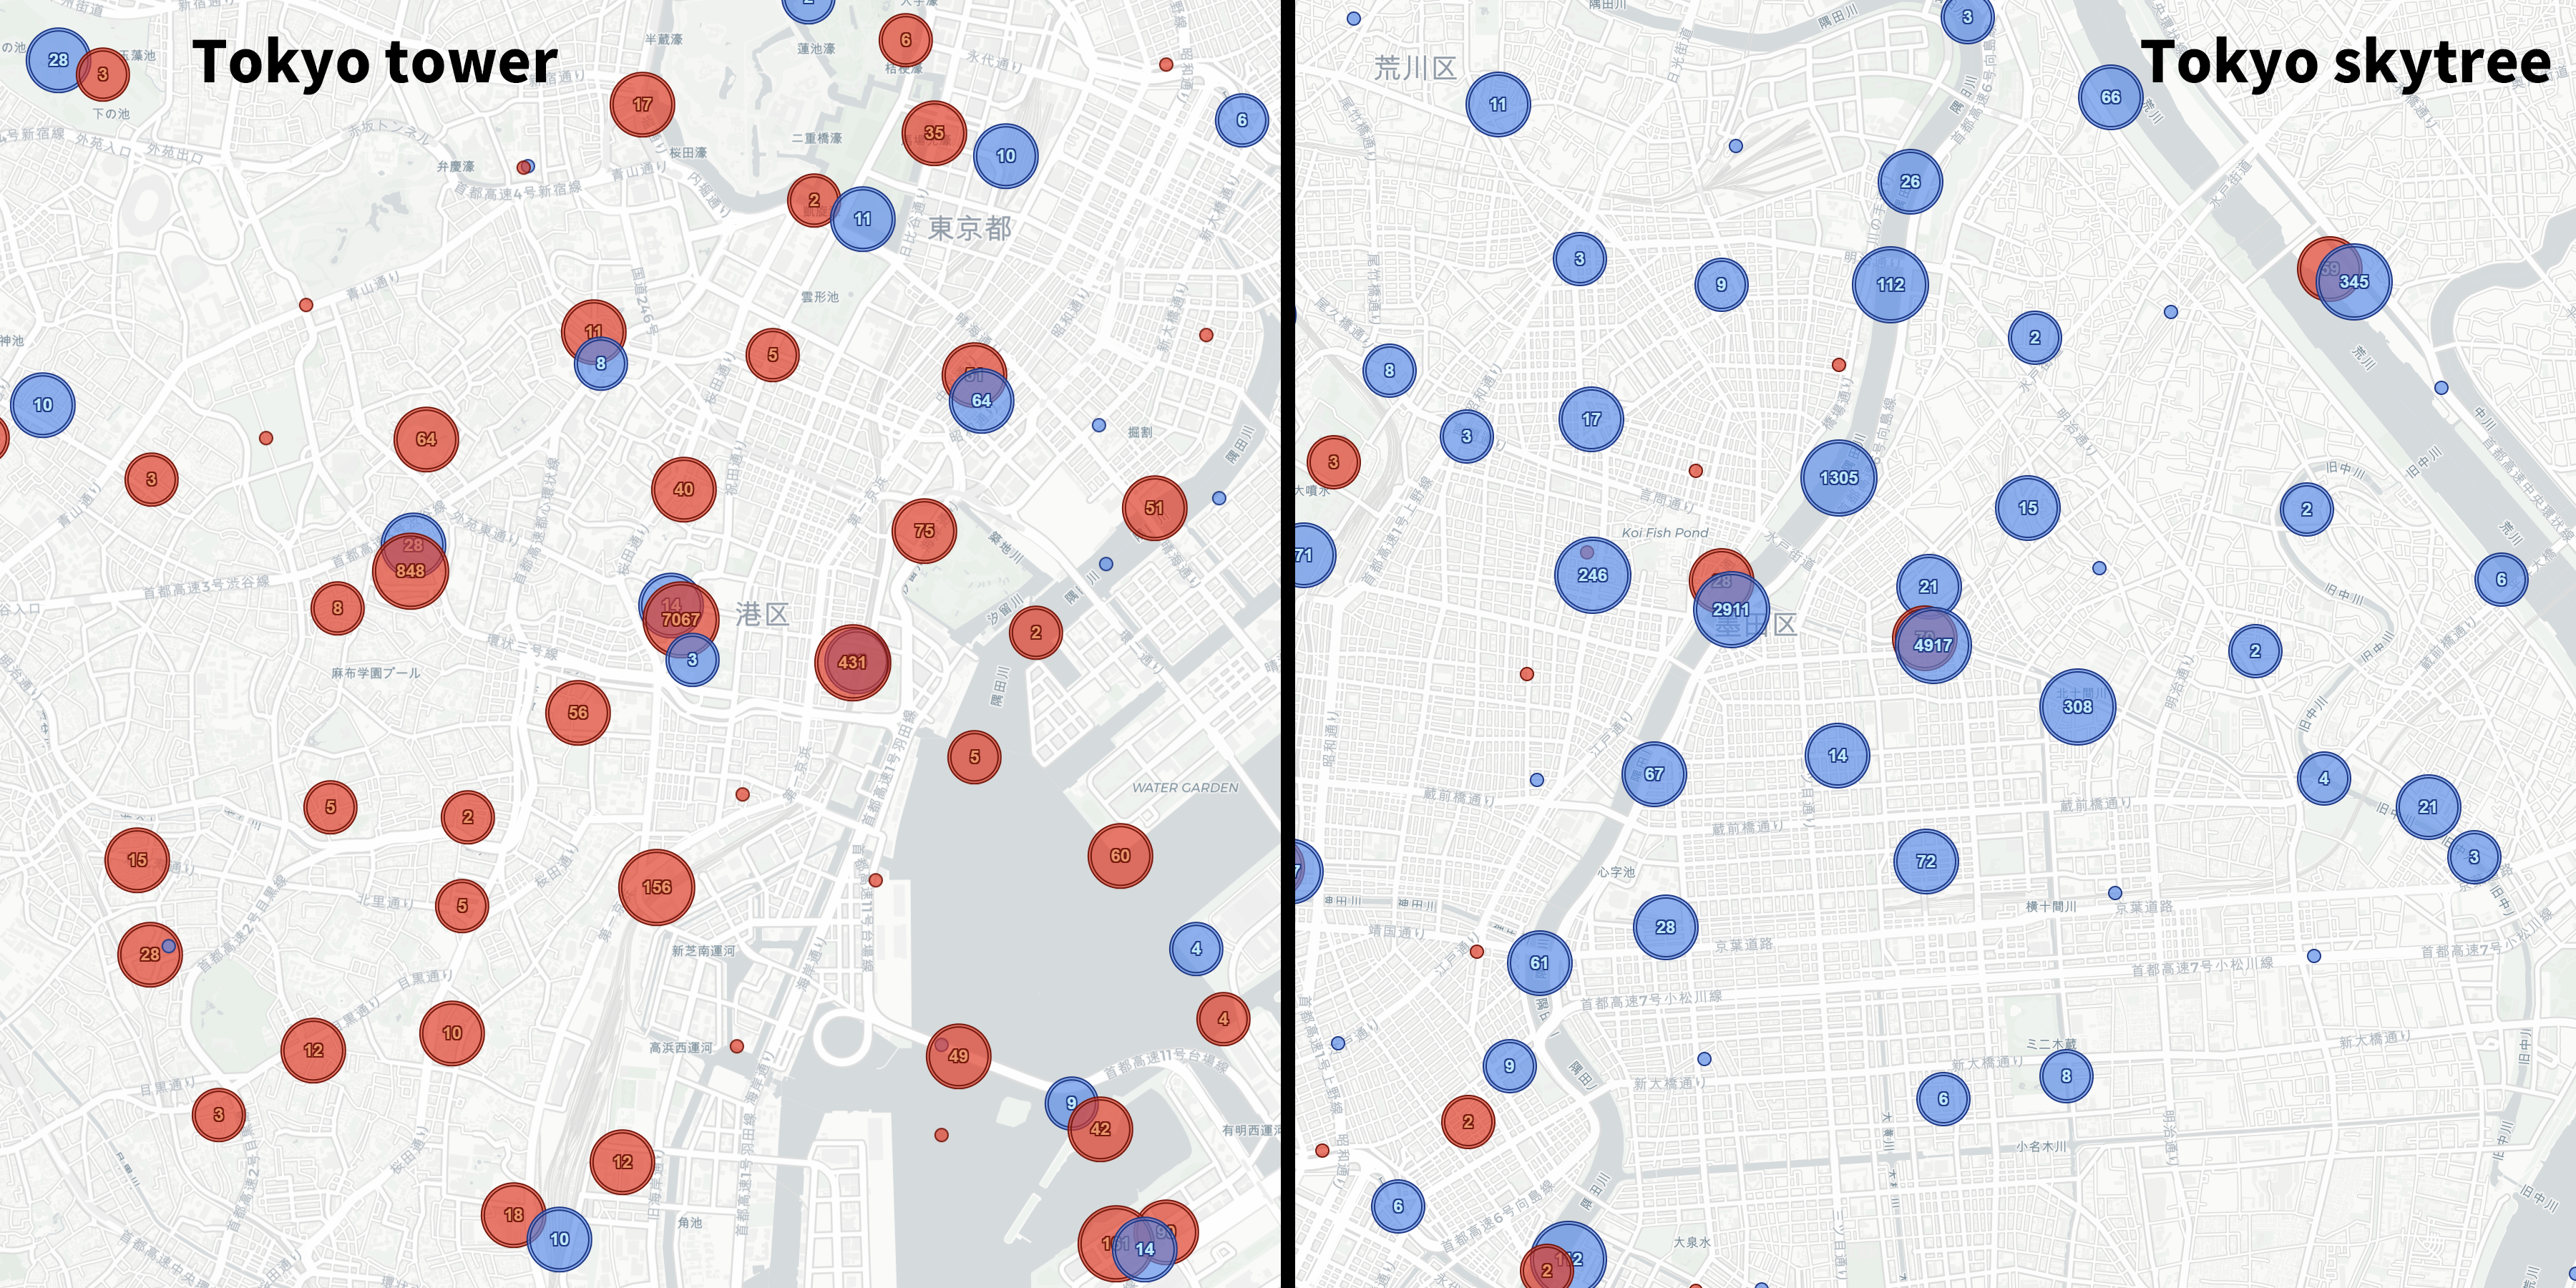
\includegraphics[width=0.9\textwidth]{figures/result_tower_marker_cluster_detail.png}
  \caption{Marker-cluster版のズームイン例}
  \label{fig:tower_marker_cluster_detail}
\end{figure}

Marker-cluster VisualizationのBulky Visualizationに対する利点は、ジオタグが密集している領域でも視認性が高い点にある.例えばスカイツリー付近で、東京タワーの写真が多数撮影されている様子が,Bulky Visualizationの結果では示されていたが、逆に東京タワー付近ではスカイツリーの写真が多数撮影されている様子が視認しづらかった.これは点群可視化が持つ典型的な問題点で、カテゴリの描画順序により、後に描画されたカテゴリが前に描画されたカテゴリを覆い隠してしまうためである.
一方でMarker-cluster可視化では、密集領域がクラスタ化されるため、カテゴリの描画順序の問題は存在するものの、マーカー数が減る事により、背後に描画されたカテゴリの分布をより目立たせる事ができるまた注目地点をズームする事(図~\ref{fig:tower_marker_cluster_detail})でより、背後のクラスタの存在は明示されるため、広域分布と局所分布の両方を効果的に探索できる点も利点である.この例から東京タワー付近にもスカイツリーのタグが付与された写真が多数撮影されている様子が把握できる.

Marker-cluster Visualizationは描画を調整するために表\ref{tab:marker_cluster_params}に示すコマンドライン引数を受け取る.
\begin{table}[h]
\centering\small
\caption{Marker-cluster Visualizationの主なコマンドライン引数}
\label{tab:marker_cluster_params} 
\begin{tabular}{llll}
\hline
引数 & 型 & 説明 & デフォルト \\ 
\hline
	\texttt{--vis-marker-cluster} & 真偽 & Marker-cluster Visualizationを有効にする & false \\
	\texttt{--v-marker-cluster-MaxClusterRadius} & 数値 & クラスタを構成する範囲(半径) & 80 \\
\hline
\end{tabular}
\end{table} 

\subsubsection{Voronoi-based Visualization}

これまでに紹介したBulkyとMarker-cluster可視化はクローリングで得られたすべての点群を元に描画する手法であった。それに対してVoronoi可視化は,点群を空間的に要約し,連続的な領域として描画する手法である.Voronoi図そのものは,種点(サイト)からの距離に基づいて空間を分割する手法であり,すべての点を使い描画する事も可能である。しかしながら、データ数が数万から数十万あるいはそれ以上の点群の場合、Voronoi図をそのまま描画すると,細かい領域が多数生成され,視覚的にノイズが多くなり,空間構造の把握が困難になる.さらに外周の不規則な領域が多くなり,計算量の増大や地図上での解釈が難しくなる問題がある.

この二つの問題を解決するために,Voronoi-based Visualizationでは,点群をHexGrid単位で空間集約し,局所的に代表的な点群を抽出してVoronoi図を生成する手法を採用している.

具体的には,まずHexGridを用いて点群を空間的に分割し,各Hexセル内で点群を集約する.次に,各Hexセル内で代表的な点群を抽出する.この際,点群の密度に基づいてサンプリングを行い,過密な領域では点群数を削減し,疎な領域では点群を保持することで,全体として均一な分布を維持する.最後に,抽出された代表点群からVoronoi図を生成し,各Voronoiセルを対応するHexセルでクリップして表示する.これにより,視覚的にノイズが少なく,解釈しやすいVoronoi図が得られる.

Voronoi-based Visualizationにおけるサイト点の抽出は,Hexセルごとに二段階の間引き処理として定式化できる.あるHexセル内の点集合を $P = \{p_i\}$ とし,各点のカテゴリを $c(p_i)$ 距離関数を地球表面上の測地距離$d(\cdot,\cdot)$とする.

まず最小サイト間隔パラメータ$r_{min}$(\texttt{--v-voronoi-MinSiteSpacingMeters})に基づき,各点の局所密度を
$$
  \operatorname{dens}(p_i)
  = \left| \left\{ p_j \in P \mid j \neq i,\ c(p_j) = c(p_i),\ d(p_i,p_j) \le r_{min} \right\} \right|
$$
として定義する.次に,点を $\operatorname{dens}(p_i)$ の大きい順に走査し,これまでに選ばれた点集合を$S_\text{spacing}$として$S_\text{spacing} = \{ p_i \in P \mid \forall p_j \in S_\text{spacing},\ c(p_j) = c(p_i) \Rightarrow d(p_i,p_j) \ge r_{min} \}$ を満たすような貪欲サンプリングを行う.この手続きにより,同一カテゴリ同士の最近距離が少なくとも $r_{min}$ となるような代表点集合 $S_\text{spacing}$ が得られ,過密なカテゴリほど代表点が強く抑制される.

次に,各Hexセル内での最大サイト数パラメータ$K_{max}$(\texttt{--v-voronoi-MaxSitesPerHex},0は無制限)に基づいてさらに点を間引く.まず$M = |S_\text{spacing}|$とし,$M \le K_{max}$の場合には追加の間引きは行わず, $S_\text{poisson} = S_\text{spacing}$ とおく.一方 $M > K_{max}$ の場合は $p = \frac{K_{max}}{M}$ とおき,各点 $p_i \in S_\text{spacing}$ を独立なベルヌーイ試行(成功確率 \(p\))で選択することにより,平均的には$ K_{max}$ 個程度の点を残すポワソン型ダウンサンプリング $S_\text{poisson}$ を構成する.実装では,この確率的間引きによって得られた点数が十分でない場合に限り,高密度領域から若干の点を補完する処理を加えている.

最終的なVoronoiサイト集合を $S$ とするとき,$K_{max} = 0$ のときは $S = S_\text{spacing}$ と定義され,$K_{max}S > 0$ のときは $S = S_\text{poisson}$ と定義される.このサイト集合 $S$ をもとに各カテゴリ毎のVoronoi図を構成し,各セルをHexセル境界でクリップして重ね合わせることで,過密域の情報量を保ちつつ,視覚的なノイズを抑えた領域ベースの可視化を実現している.

まとめると、Voronoi-based Visualizationは,各Hexセル内で最小サイト間隔以下の点を、カテゴリの出現割合を尊重しつつ間引く事で、過度にVoronoiセルが細分化されるのを防ぎ、加えて各Hexセル内で指定された最大サイト数によりポワソン型ダウンサンプリングを行い代表点を抽出し,Voronoi図を生成する手法である.これにより,視覚的にノイズが少なく解釈しやすいVoronoi図が得られ,ジオタグ付き画像の空間分布の特徴を効果的に把握できる. 

前述までと同様に東京タワーとスカイツリーの撮影位置分布をVoronoi可視化で表現した例を図~\ref{fig:tower_voronoi}に示す.

\begin{figure}[h]
  \centering
  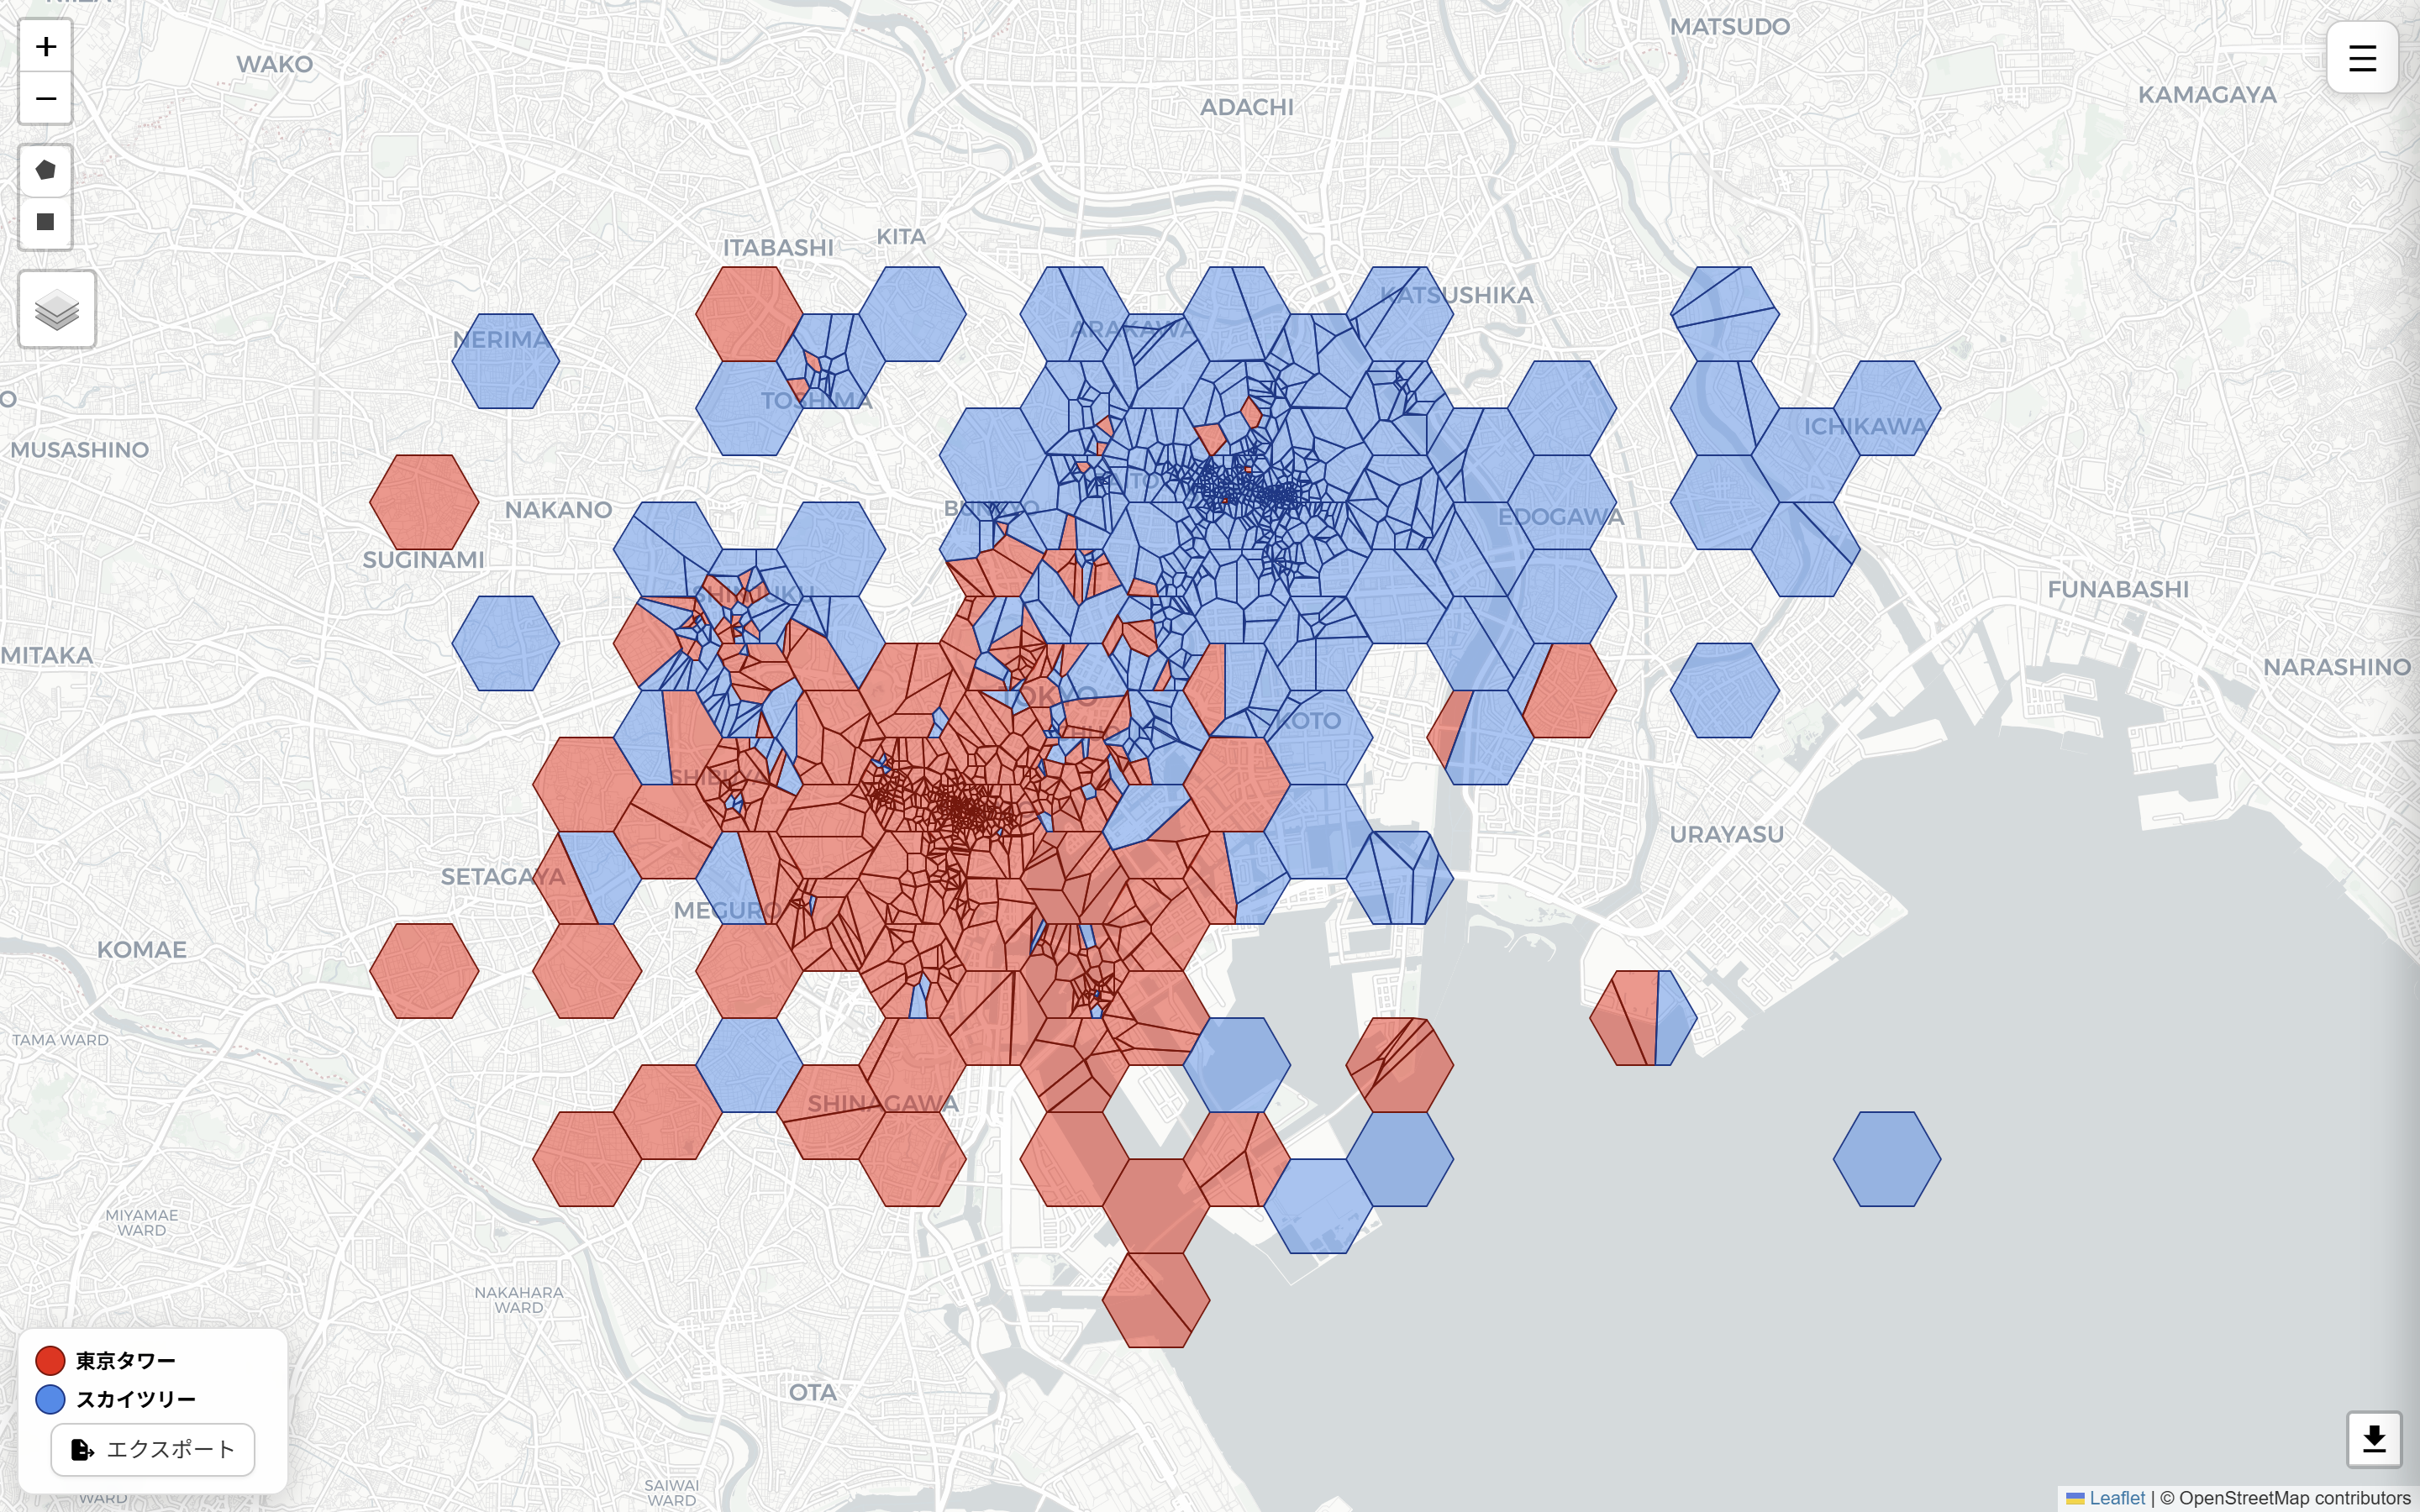
\includegraphics[width=0.9\textwidth]{figures/result_tower_voronoi.png}
  \caption{東京タワーとスカイツリーの撮影位置分布の可視化例(voronoi版)}
  \label{fig:tower_voronoi}
\end{figure}

この図に表れているように、東京タワー近辺、スカイツリー近辺はVoronoiセルが細かく分割されており、撮影位置が集中している様子が視覚的に把握できる.一方で両ランドマークから離れた地域ではVoronoiセルが大きくなっており、撮影位置が疎である様子が視覚的に把握できる.ただし、Marker-cluster Visualizationとは異なり、両タワーの近辺で他方のタワーの写真が撮影されているが、両の差は顕著であり、ダウンサンプリングの過程で消えてしまっている様子が視覚的に把握できる.
コマンドは次のとおりである。

\begin{commandline}
npx -y -p splatone@latest crawler -p flickr \
-k "東京タワー#FA0000=tokyotower,東京タワー|スカイツリー#2B89EE=skytree,スカイツリー"  \
--vis-voronoi --p-flickr-APIKEY="aaaaaaaaaaaaaaaaaaaaaaaaaaaaaaaaaaaaaaaaa"
\end{commandline}

Voronoi Visualizationは描画を調整するために表\ref{tab:voronoi_params}に示すコマンドライン引数を受け取る.

\begin{table}[h]
\centering\small
\caption{Voronoi Visualizationの主なコマンドライン引数}
\label{tab:voronoi_params}
\begin{tabular}{llll}
\hline
引数 & 型 & 説明 & デフォルト \\
\hline
	\texttt{--vis-voronoi} & 真偽 & Voronoi Visualizationを有効にする & false \\
	\texttt{--v-voronoi-MaxSitesPerHex} & 数値 & 各Hex内で残す最大サイト数(0=無制限) & 0 \\
	\texttt{--v-voronoi-MinSiteSpacingMeters} & 数値 & サイト間の最小距離[メートル] & 50 \\
\hline
\end{tabular}
\end{table}

\subsubsection{Pie-charts Visualization}
Pie-charts可視化では,空間を一定のグリッドまたはクラスタで分割し,各セル内のカテゴリ比率を円グラフとして表示する.また、円グラフの大きさをセル内の画像数に比例させることで,カテゴリ分布とセル内密度の両方を同時に把握できる.

これまで同様に東京タワーとスカイツリーの撮影位置分布をPie-charts可視化で表現した例を図~\ref{fig:tower_pie_charts}に示す.

\begin{figure}[h]
  \centering
  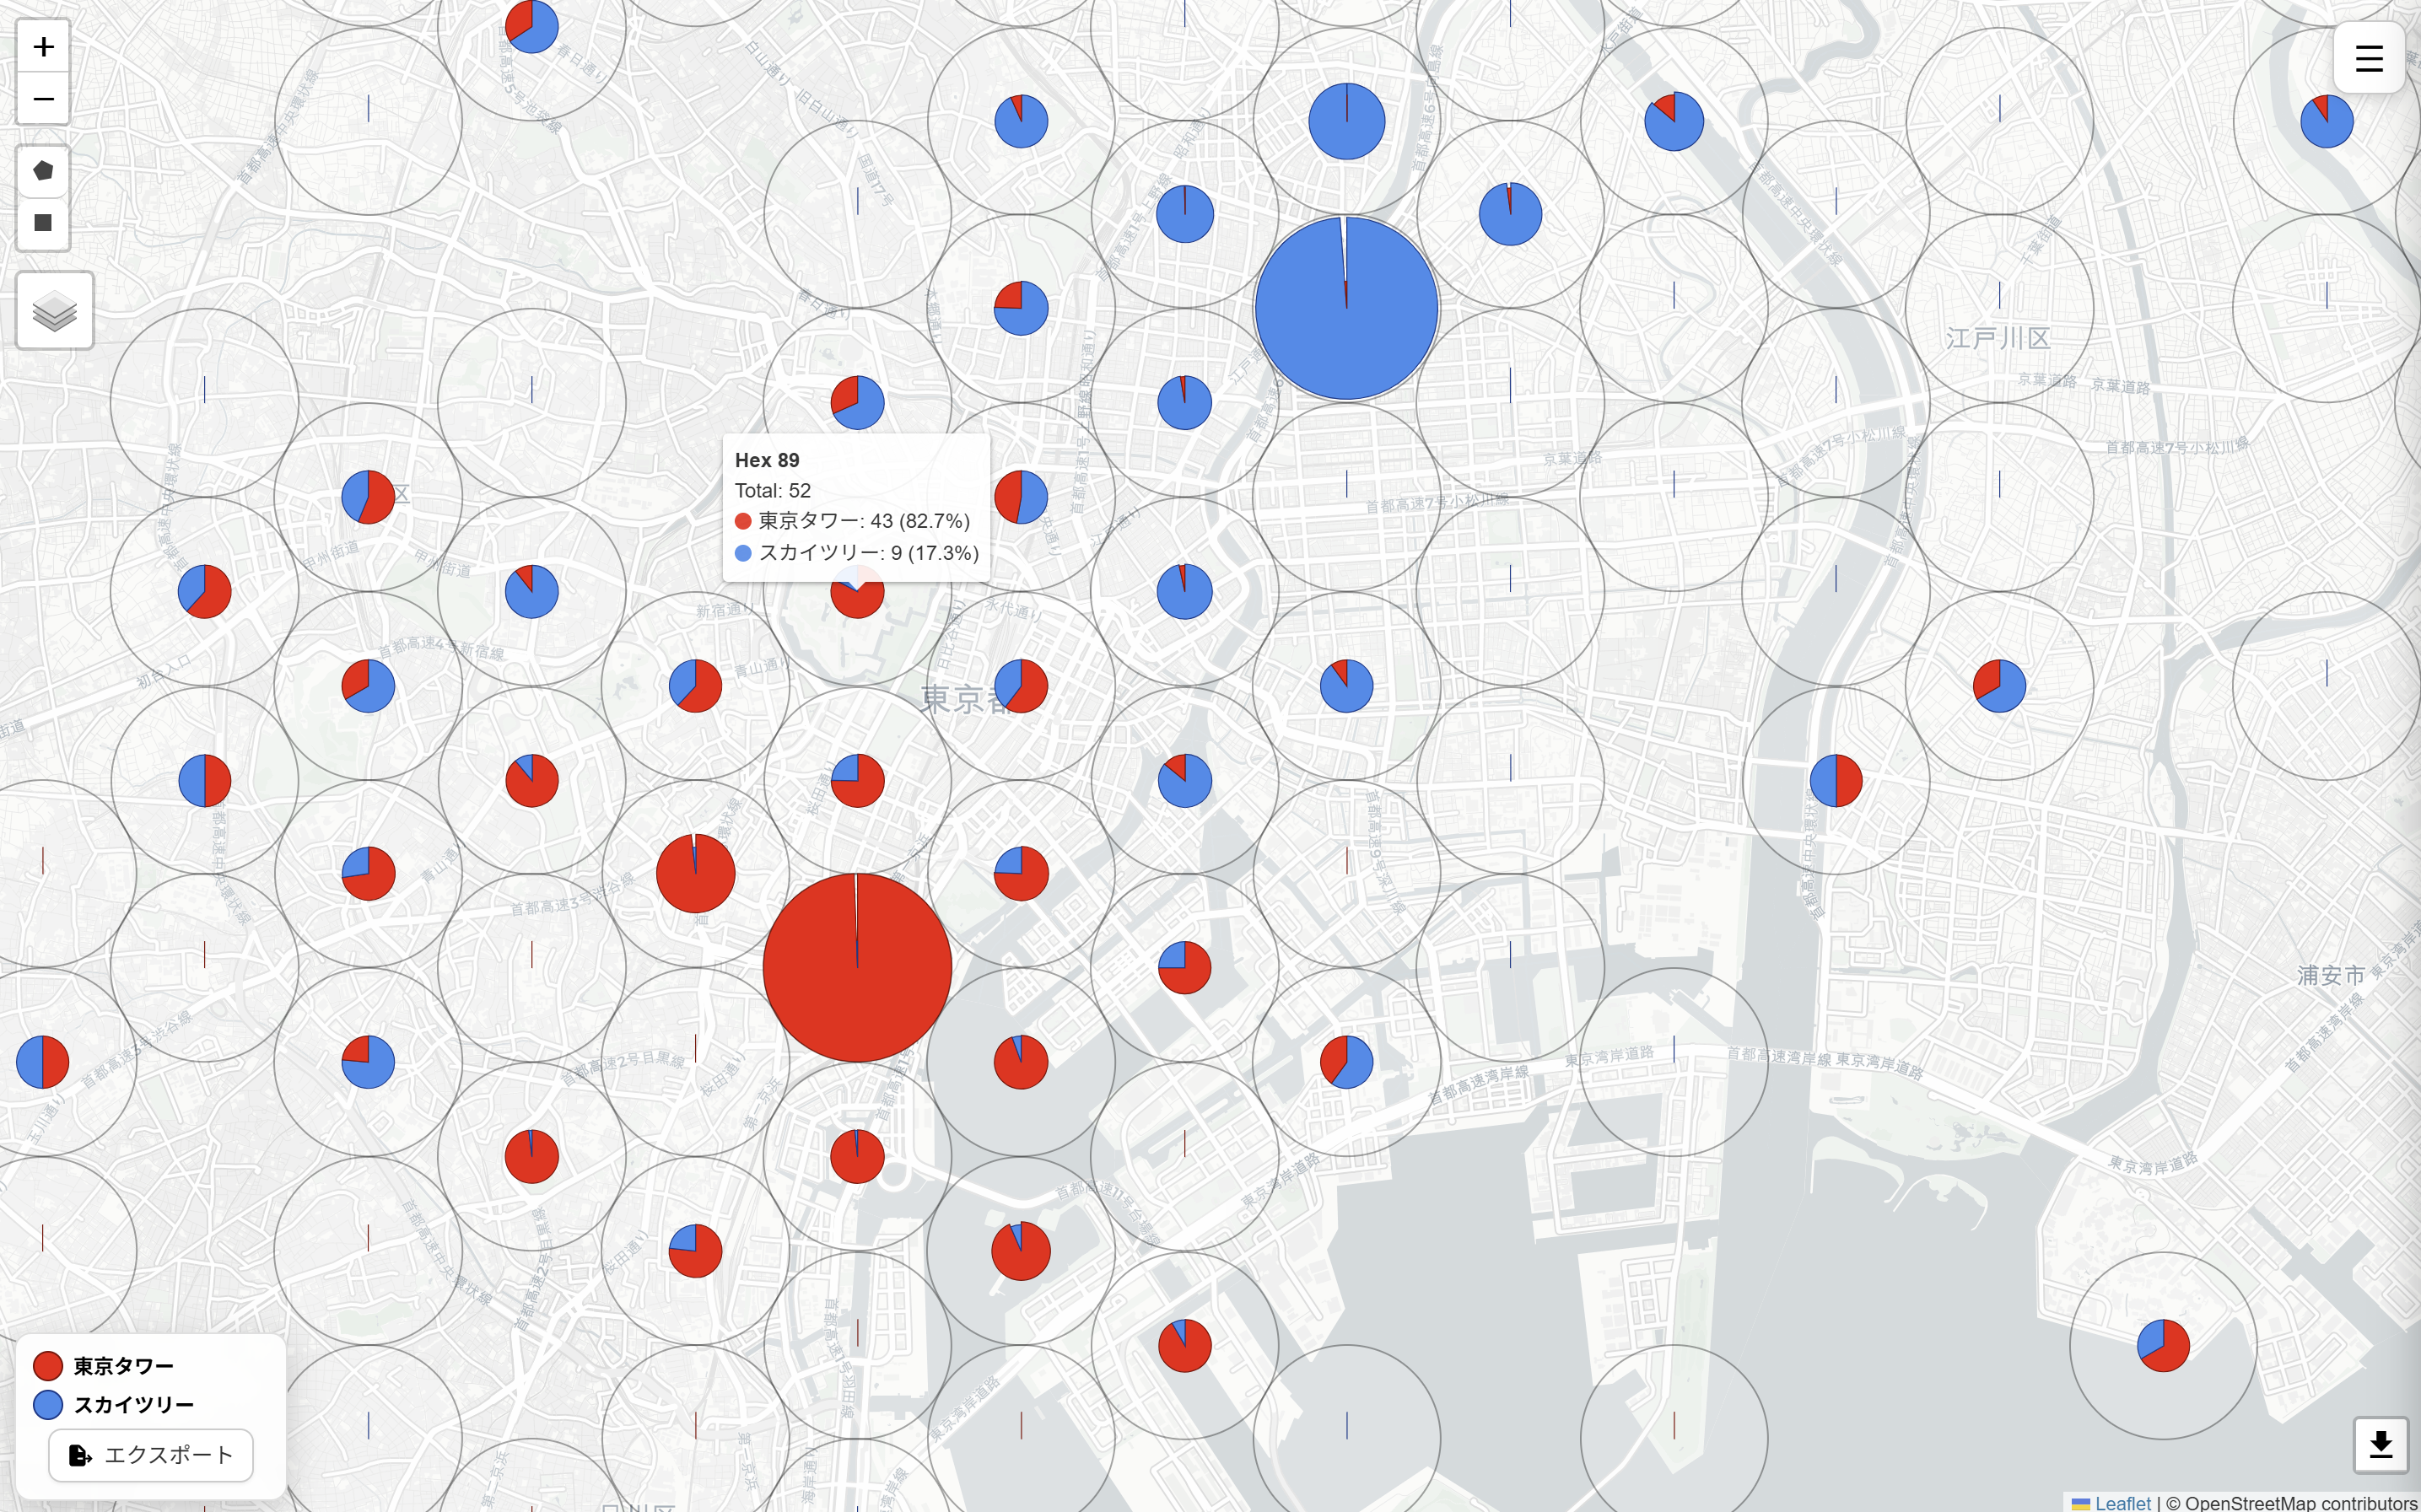
\includegraphics[width=0.9\textwidth]{figures/result_tower_pie_charts.png}
  \caption{東京タワーとスカイツリーの撮影位置分布の可視化例(pie-charts版)}
  \label{fig:tower_pie_charts}
\end{figure}
この図に表れているように、東京タワー近辺、スカイツリー近辺では円グラフが大きく描画されており、撮影位置が集中している様子が視覚的に把握できる.また、両ランドマークから離れた地域では円グラフが小さくなっており、撮影位置が疎である様子が視覚的に把握できる.さらに、各円グラフ内の色の割合から、各地域でどのカテゴリの写真が多く撮影されているかも把握できる.例えば、東京タワー近辺では赤色(東京タワーカテゴリ)が優勢であり、スカイツリー近辺では青色(スカイツリーカテゴリ)が優勢である様子が視覚的に把握できる.

コマンドは次のとおりである。
\begin{commandline}
npx -y -p splatone@latest crawler -p flickr \ 
-k "東京タワー#FA0000=tokyotower,東京タワー|スカイツリー#2B89EE=skytree,スカイツリー"  \
--vis-pie-charts --p-flickr-APIKEY="aaaaaaaaaaaaaaaaaaaaaaaaaaaaaaaaaaaaaaaaa"
\end{commandline}

Pie-charts Visualizationは描画を調整するために表\ref{tab:pie_charts_params}に示すコマンドライン引数を受け取る.

\begin{table}[h]
\centering\small
\caption{Pie-charts Visualizationの主なコマンドライン引数}
\label{tab:pie_charts_params}
\begin{tabular}{llll}
\hline
引数 & 型 & 説明 & デフォルト \\
\hline
  \texttt{--vis-pie-charts} & 真偽 & Pie-charts Visualizationを有効にする & false \\
  \texttt{--v-pie-charts-MaxRadiusScale} & 数値 & Hex内接円半径に対する最大半径スケール(0–1.5) & 0.9 \\
  \texttt{--v-pie-charts-MinRadiusScale} & 数値 & 最大半径に対する最小半径スケール(0–1) & 0.25 \\
  \texttt{--v-pie-charts-StrokeWidth} & 数値 & Pie Chart輪郭線の太さ(px) & 1 \\
  \texttt{--v-pie-charts-BackgroundOpacity} & 数値 & 最大半径ガイドリングの透明度(0–1) & 0.2 \\
\hline
\end{tabular}
\end{table}

\subsubsection{Majority-hex Visualization}

Pie-charts Visualizationでは各セル内のカテゴリ比率は効果的に把握できるものの、地図上に円グラフを重ねる構成は地理的な特徴を地図上で直感的に把握するという本ツールの目的とは方向性が異なっている。

一方で地理的な特徴をカテゴリ色を使って直感的に把握する手法としてヒートマップがある。Splatone CrawlerではHexGridを単位としたヒートマップの一種であるMajority-hex Visualizationを提供している。

Majority Hex可視化では,地理空間を等間隔のHexGridに分割し,各セル内で最も頻度の高いカテゴリを求めて、全体におけるそのセルの割合を透明度として表示する.これにより,カテゴリごとの支配的な空間分布がモザイク状に示され,かつ範囲全体において分布が集中している箇所をより濃く描く事で地理的な分布を俯瞰しやすくなる.図~\ref{fig:tower_majority_hex_simple}に,東京タワーとスカイツリーの撮影位置分布をMajority-hex可視化で表現した例を示す.

\begin{figure}[h]
  \centering
  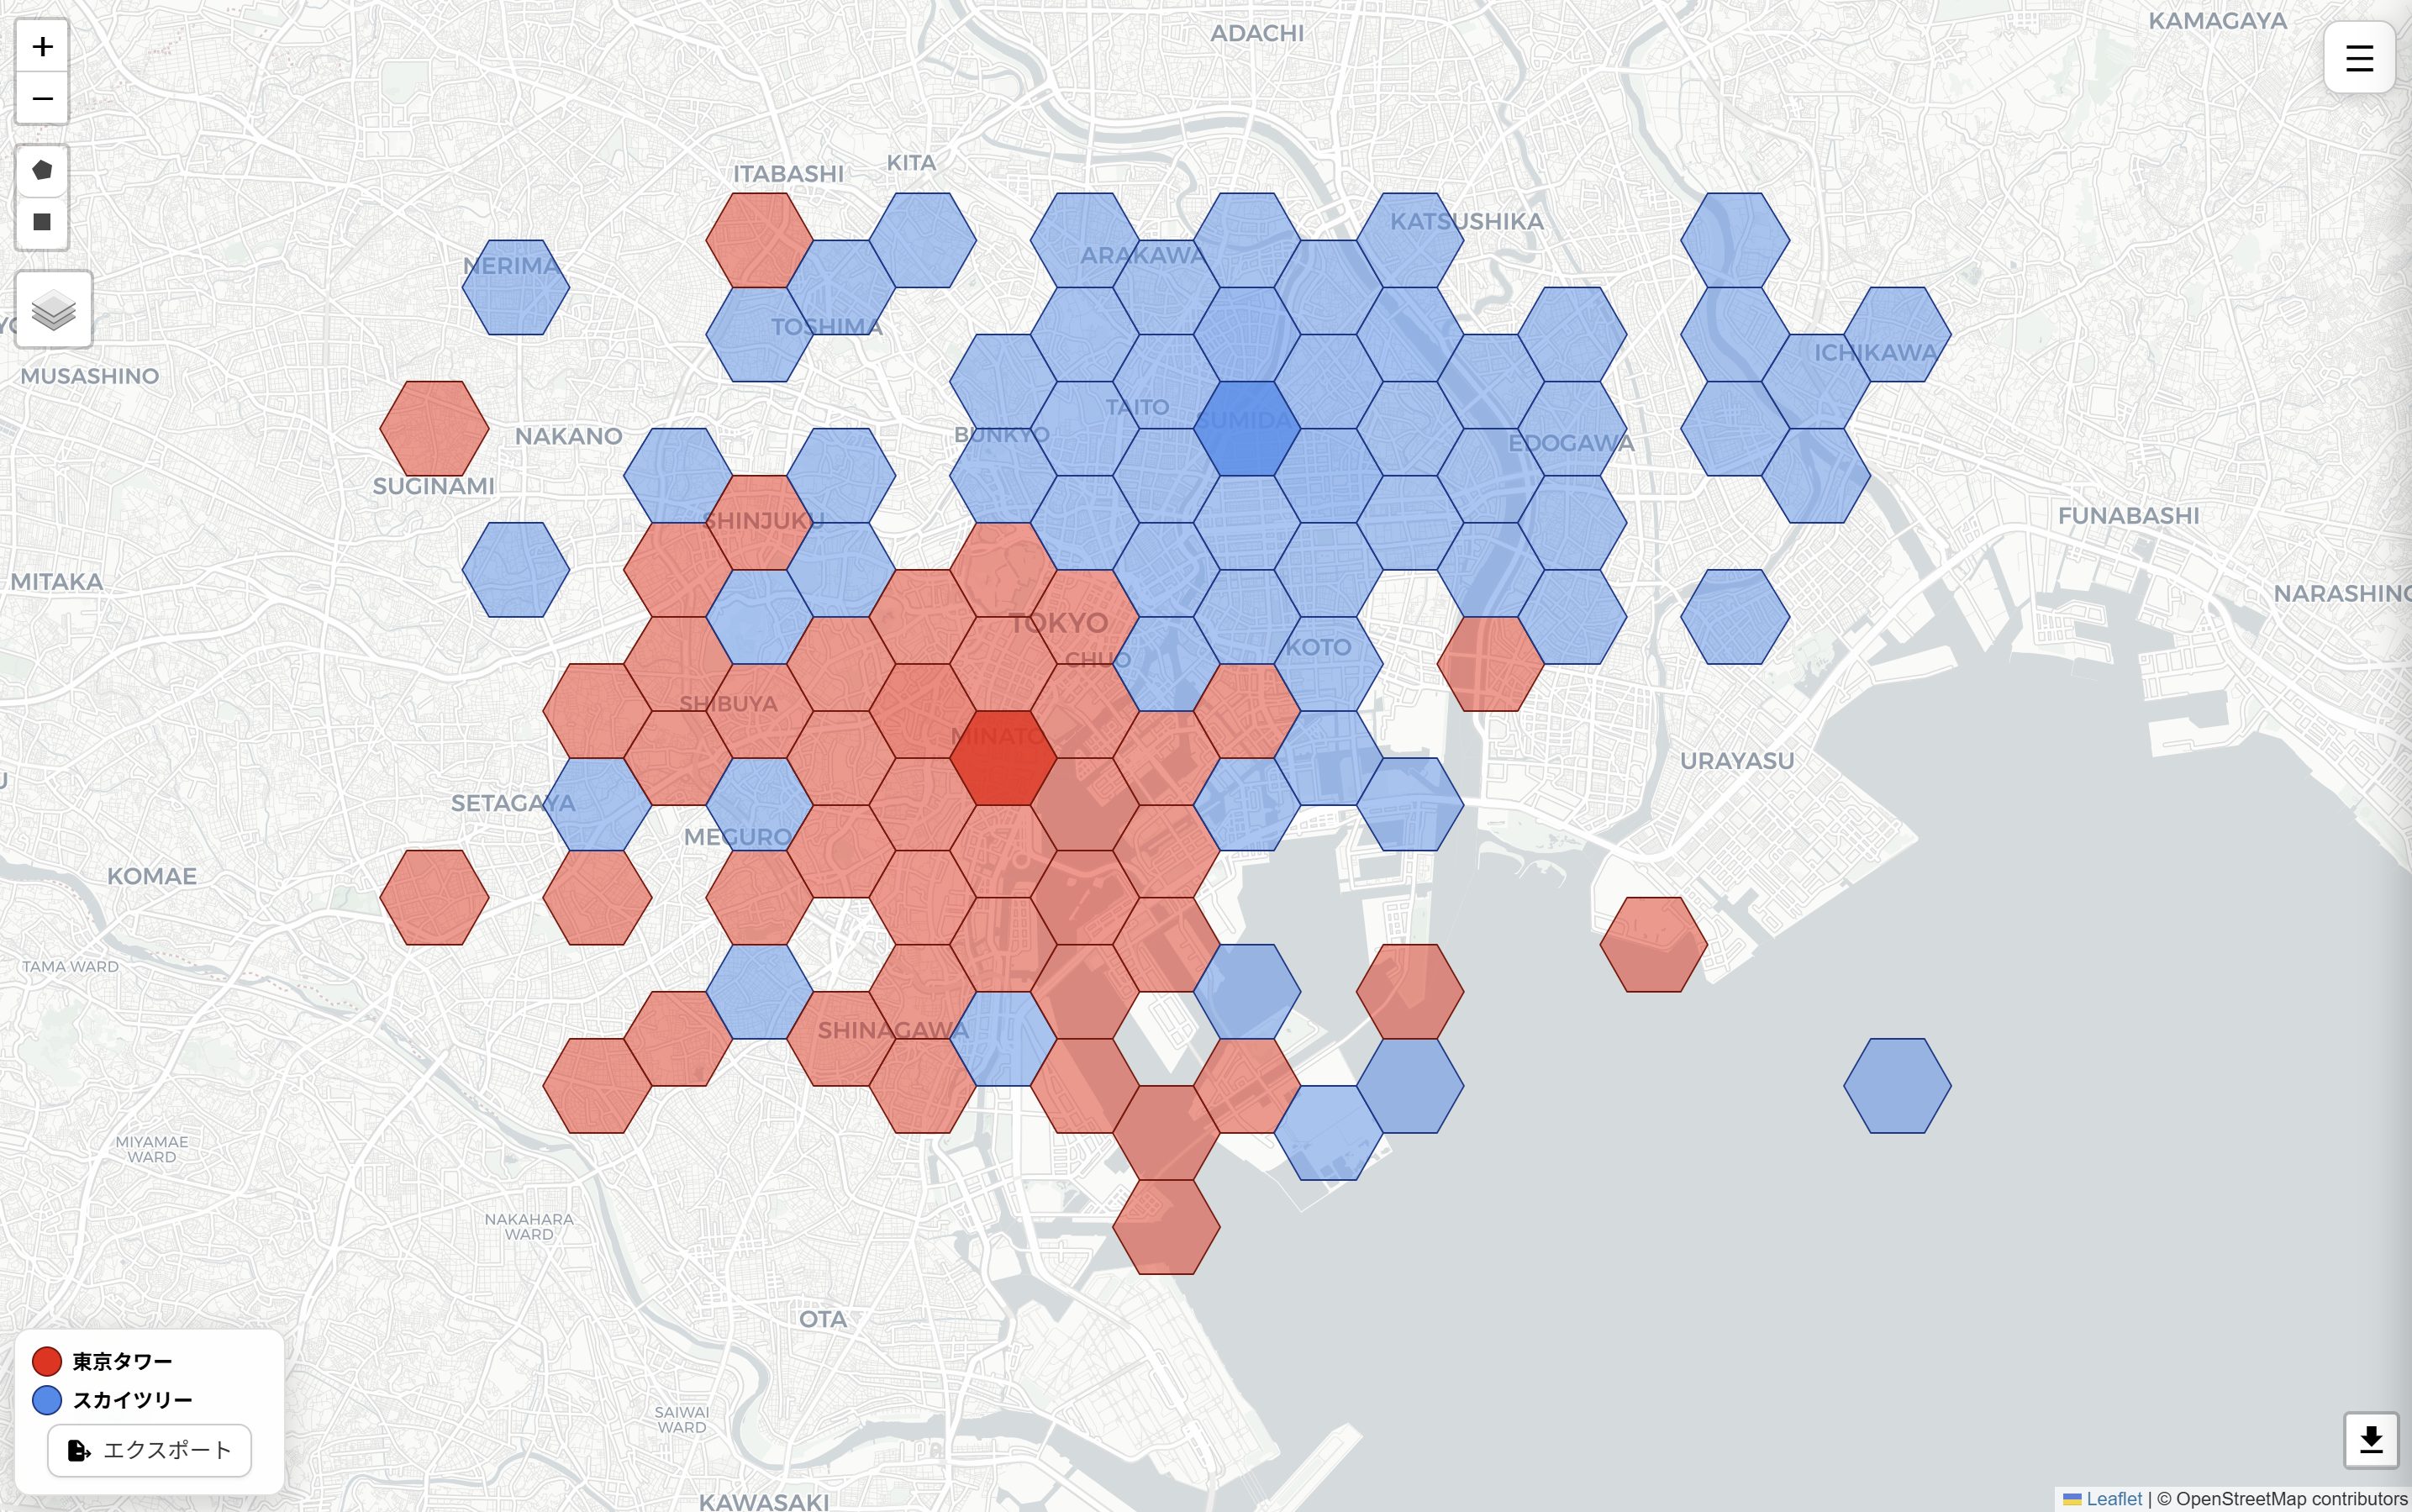
\includegraphics[width=0.9\textwidth]{figures/result_tower_majority_hex.png}
  \caption{東京タワーとスカイツリーの撮影位置分布の可視化例(majority-hex版,単純表示)}
  \label{fig:tower_majority_hex_simple}
\end{figure}

東京タワーを中心に赤色のHexセルが広がっており、スカイツリーを中心に青色のHexセルが広がっている様子が視覚的に把握できる.また、両ランドマークから離れた地域ではHexセルが薄く描画されており、撮影位置が疎である様子が視覚的に把握できる.

ここで、単純に各セルの最多カテゴリのみをもちいて彩色すると,セル内のカテゴリ分布の多様性が失われ,情報が欠落する問題について考える.
この問題を解決するために,Majority-hex Visualizationでは,各セル内のカテゴリ頻度に基づいて六角形を6個の三角形に分割彩色するオプション\texttt{--v-majority-hex-Hexapartite}を提供している.例えば,あるHexセル内でカテゴリAが60\%,カテゴリBが30\%,カテゴリCが10\%であった場合、まず比率×6の整数部分を割り当てると,それぞれ3,1,0となり,合計4つの三角形が割り当てられる.残りの2つの三角形は,比率の小数部分に基づいてカテゴリAに1つ,カテゴリBに1つ割り当てられる.
このようにして,各セル内のカテゴリ頻度を反映した分割彩色が行われる.図~\ref{fig:tower_majority_hex_Hexapartite}に,六角形分割彩色オプションを有効にした場合のMajority-hex可視化の例を示す.

\begin{figure}[h]
  \centering
  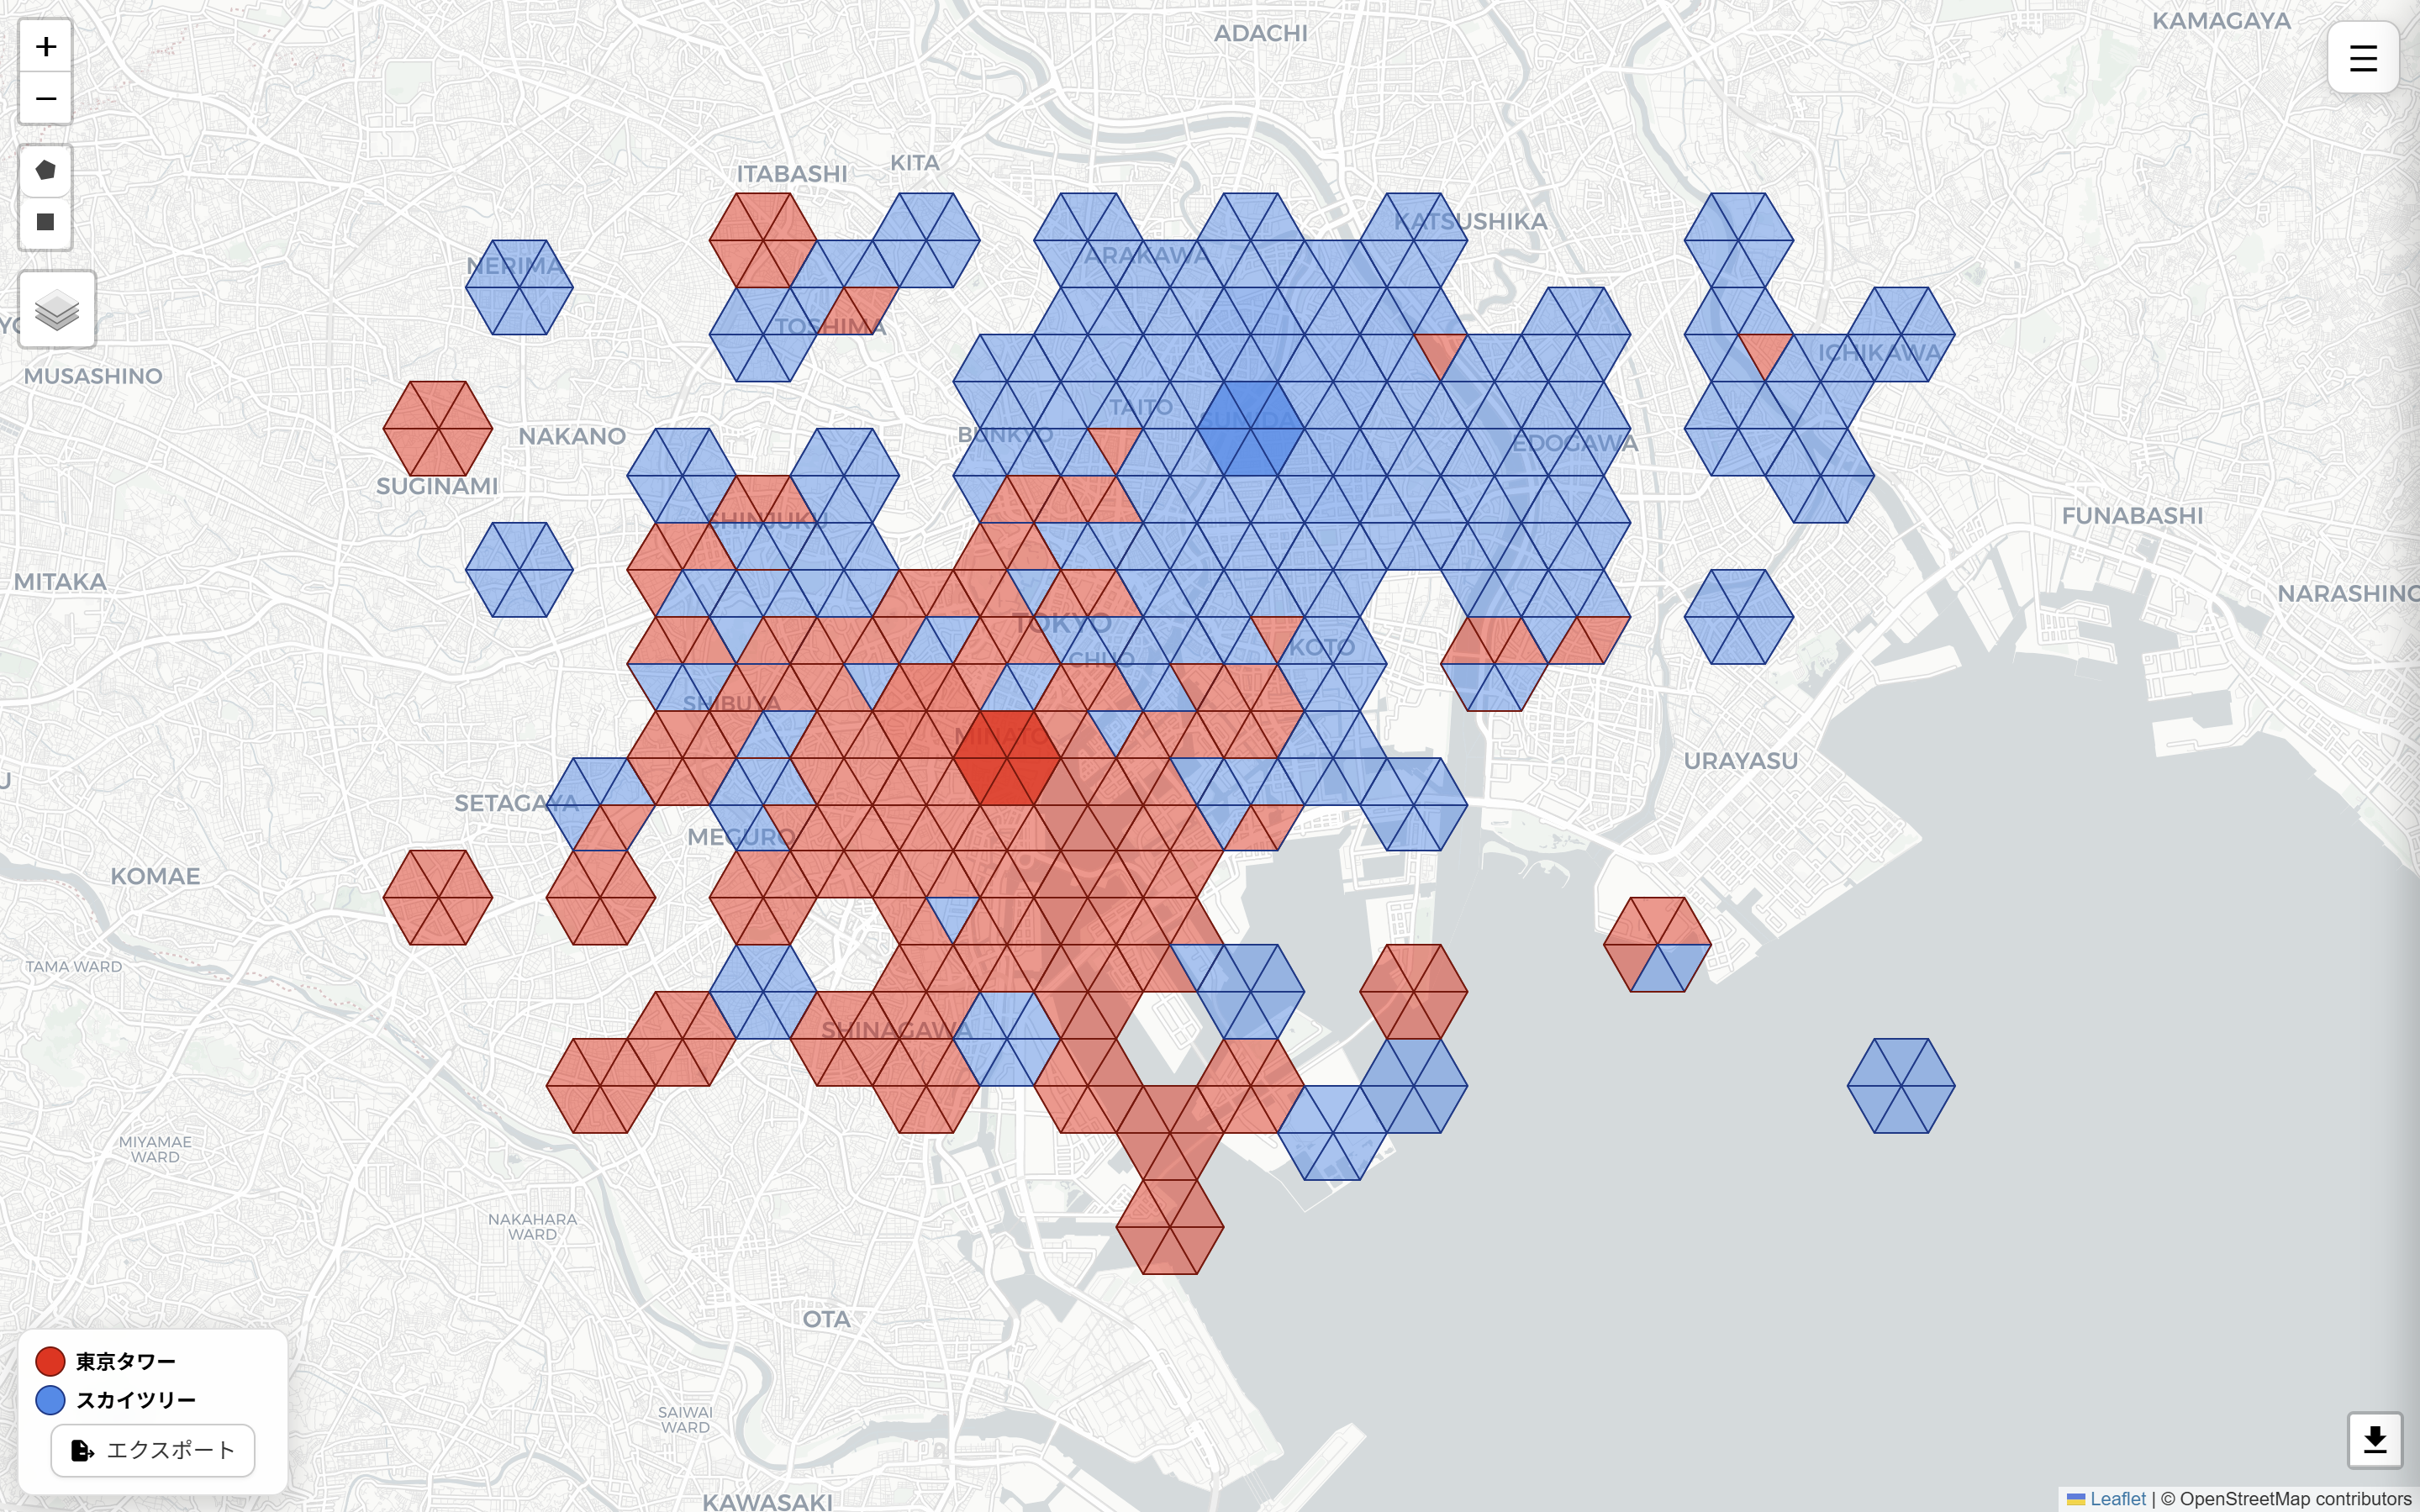
\includegraphics[width=0.9\textwidth]{figures/result_tower_majority_hex_hexapartite.png}
  \caption{東京タワーとスカイツリーの撮影位置分布の可視化例(majority-hex版,六角形分割彩色)}
  \label{fig:tower_majority_hex_Hexapartite}
\end{figure}

図~\ref{fig:tower_majority_hex_simple}に比べて,図~\ref{fig:tower_majority_hex_Hexapartite}では各Hexセル内のカテゴリ分布の多様性と距離によるグラデーションがより豊かに表現されている様子が視覚的に把握できる.

この例示に利用したコマンドを以下に示す.なお、APIKEYは各自で取得したものに置き換える必要がある.
\begin{commandline}
npx -y -p splatone@latest crawler -p flickr \
-k "東京タワー#FA0000=tokyotower,東京タワー|スカイツリー#2B89EE=skytree,スカイツリー"  \
--vis-majority-hex --v-majority-hex-Hexapartite \ 
--p-flickr-APIKEY="aaaaaaaaaaaaaaaaaaaaaaaaaaaaaaaaaaaaaaaaa"
\end{commandline}


Majority-hex Visualizationは描画を調整するために表\ref{tab:majority_hex_params}に示すコマンドライン引数を受け取る.

\begin{table}[h]
\centering\small
\caption{Majority-hex Visualizationの主なコマンドライン引数}
\label{tab:majority_hex_params}
\begin{tabular}{llll}
\hline
引数 & 型 & 説明 & デフォルト \\
\hline
  \texttt{--vis-majority-hex} & 真偽 & Majority-hex Visualizationを有効にする & false \\
  \texttt{--v-majority-hex-Hexapartite} & 真偽 & Hex内カテゴリ頻度に応じて六角形を分割色彩 & false \\
  \texttt{--v-majority-hex-HexOpacity} & 数値 & 六角形の線の透明度 & 1 \\
  \texttt{--v-majority-hex-HexWeight} & 数値 & 六角形の線の太さ & 1 \\
  \texttt{--v-majority-hex-MaxOpacity} & 数値 & 正規化後の最大塗り透明度 & 0.9 \\
  \texttt{--v-majority-hex-MinOpacity} & 数値 & 正規化後の最小塗り透明度 & 0.5 \\
\hline
\end{tabular}
\end{table}

\subsubsection{Heatmap Visualization}
グリッドベースのヒートマップではなく,連続的な密度場としてジオタグ付き写真の分布を可視化する手法としてHeatmap Visualizationを提供している.

Heatmap Visualizationでは,位置情報付き写真の点群を連続的な密度場として近似し,その値を色の濃淡として地図上に描画する.Splatone Crawler では,地点集合 $\{p_i\}_{i=1}^n$ に対する二次元カーネル密度推定(Kernel Density Estimation; KDE)\cite{silverman1986density} を用いて,位置 $x$ における密度 $\hat f(x)$ を
$$
  \hat f(x)
  = \frac{1}{n h^2} \sum_{i=1}^n K\left( \frac{\lVert x - p_i \rVert}{h} \right)
$$
と定義する.ここで $K(\cdot)$ は半径 1 の球対称カーネル関数(実装ではガウシアンに近い平滑カーネル),$h$ はバンド幅(スムージング半径)であり,\texttt{--v-heat-Radius} と \texttt{--v-heat-Units} により地理座標系上の距離として指定される.点 $p_i$ の寄与は距離 $\lVert x - p_i \rVert$ が $h$ を超えると急速に減衰し,遠方の点はほとんど影響を与えない.

実装上は,可視化領域を長辺方向 \texttt{--v-dbscan-GridSize} と同様のグリッド解像度に分割し,各グリッド中心 $x_g$ ごとに上記の $\hat f(x_g)$ を近似的に計算することで密度ラスタを生成している.その後,得られた密度値を最大値で正規化し,\texttt{--v-heat-MinOpacity} から \texttt{--v-heat-MaxOpacity} の間に線形マッピングすることで,低密度領域は透過,高密度領域は不透明に近い表示となる.上限値は \texttt{--v-heat-MaxValue} を指定しない場合,自動的にデータに基づき推定される.また,近傍点数が \texttt{--v-heat-WeightThreshold} 未満の場所は描画対象から除外されるため,孤立した撮影点によるノイズ的なヒートスポットの発生を抑制できる.

図~\ref{fig:tower_heatmap}に,東京タワーとスカイツリーの撮影位置分布をHeatmap可視化で表現した例を示す.
\begin{figure}[h]
  \centering
  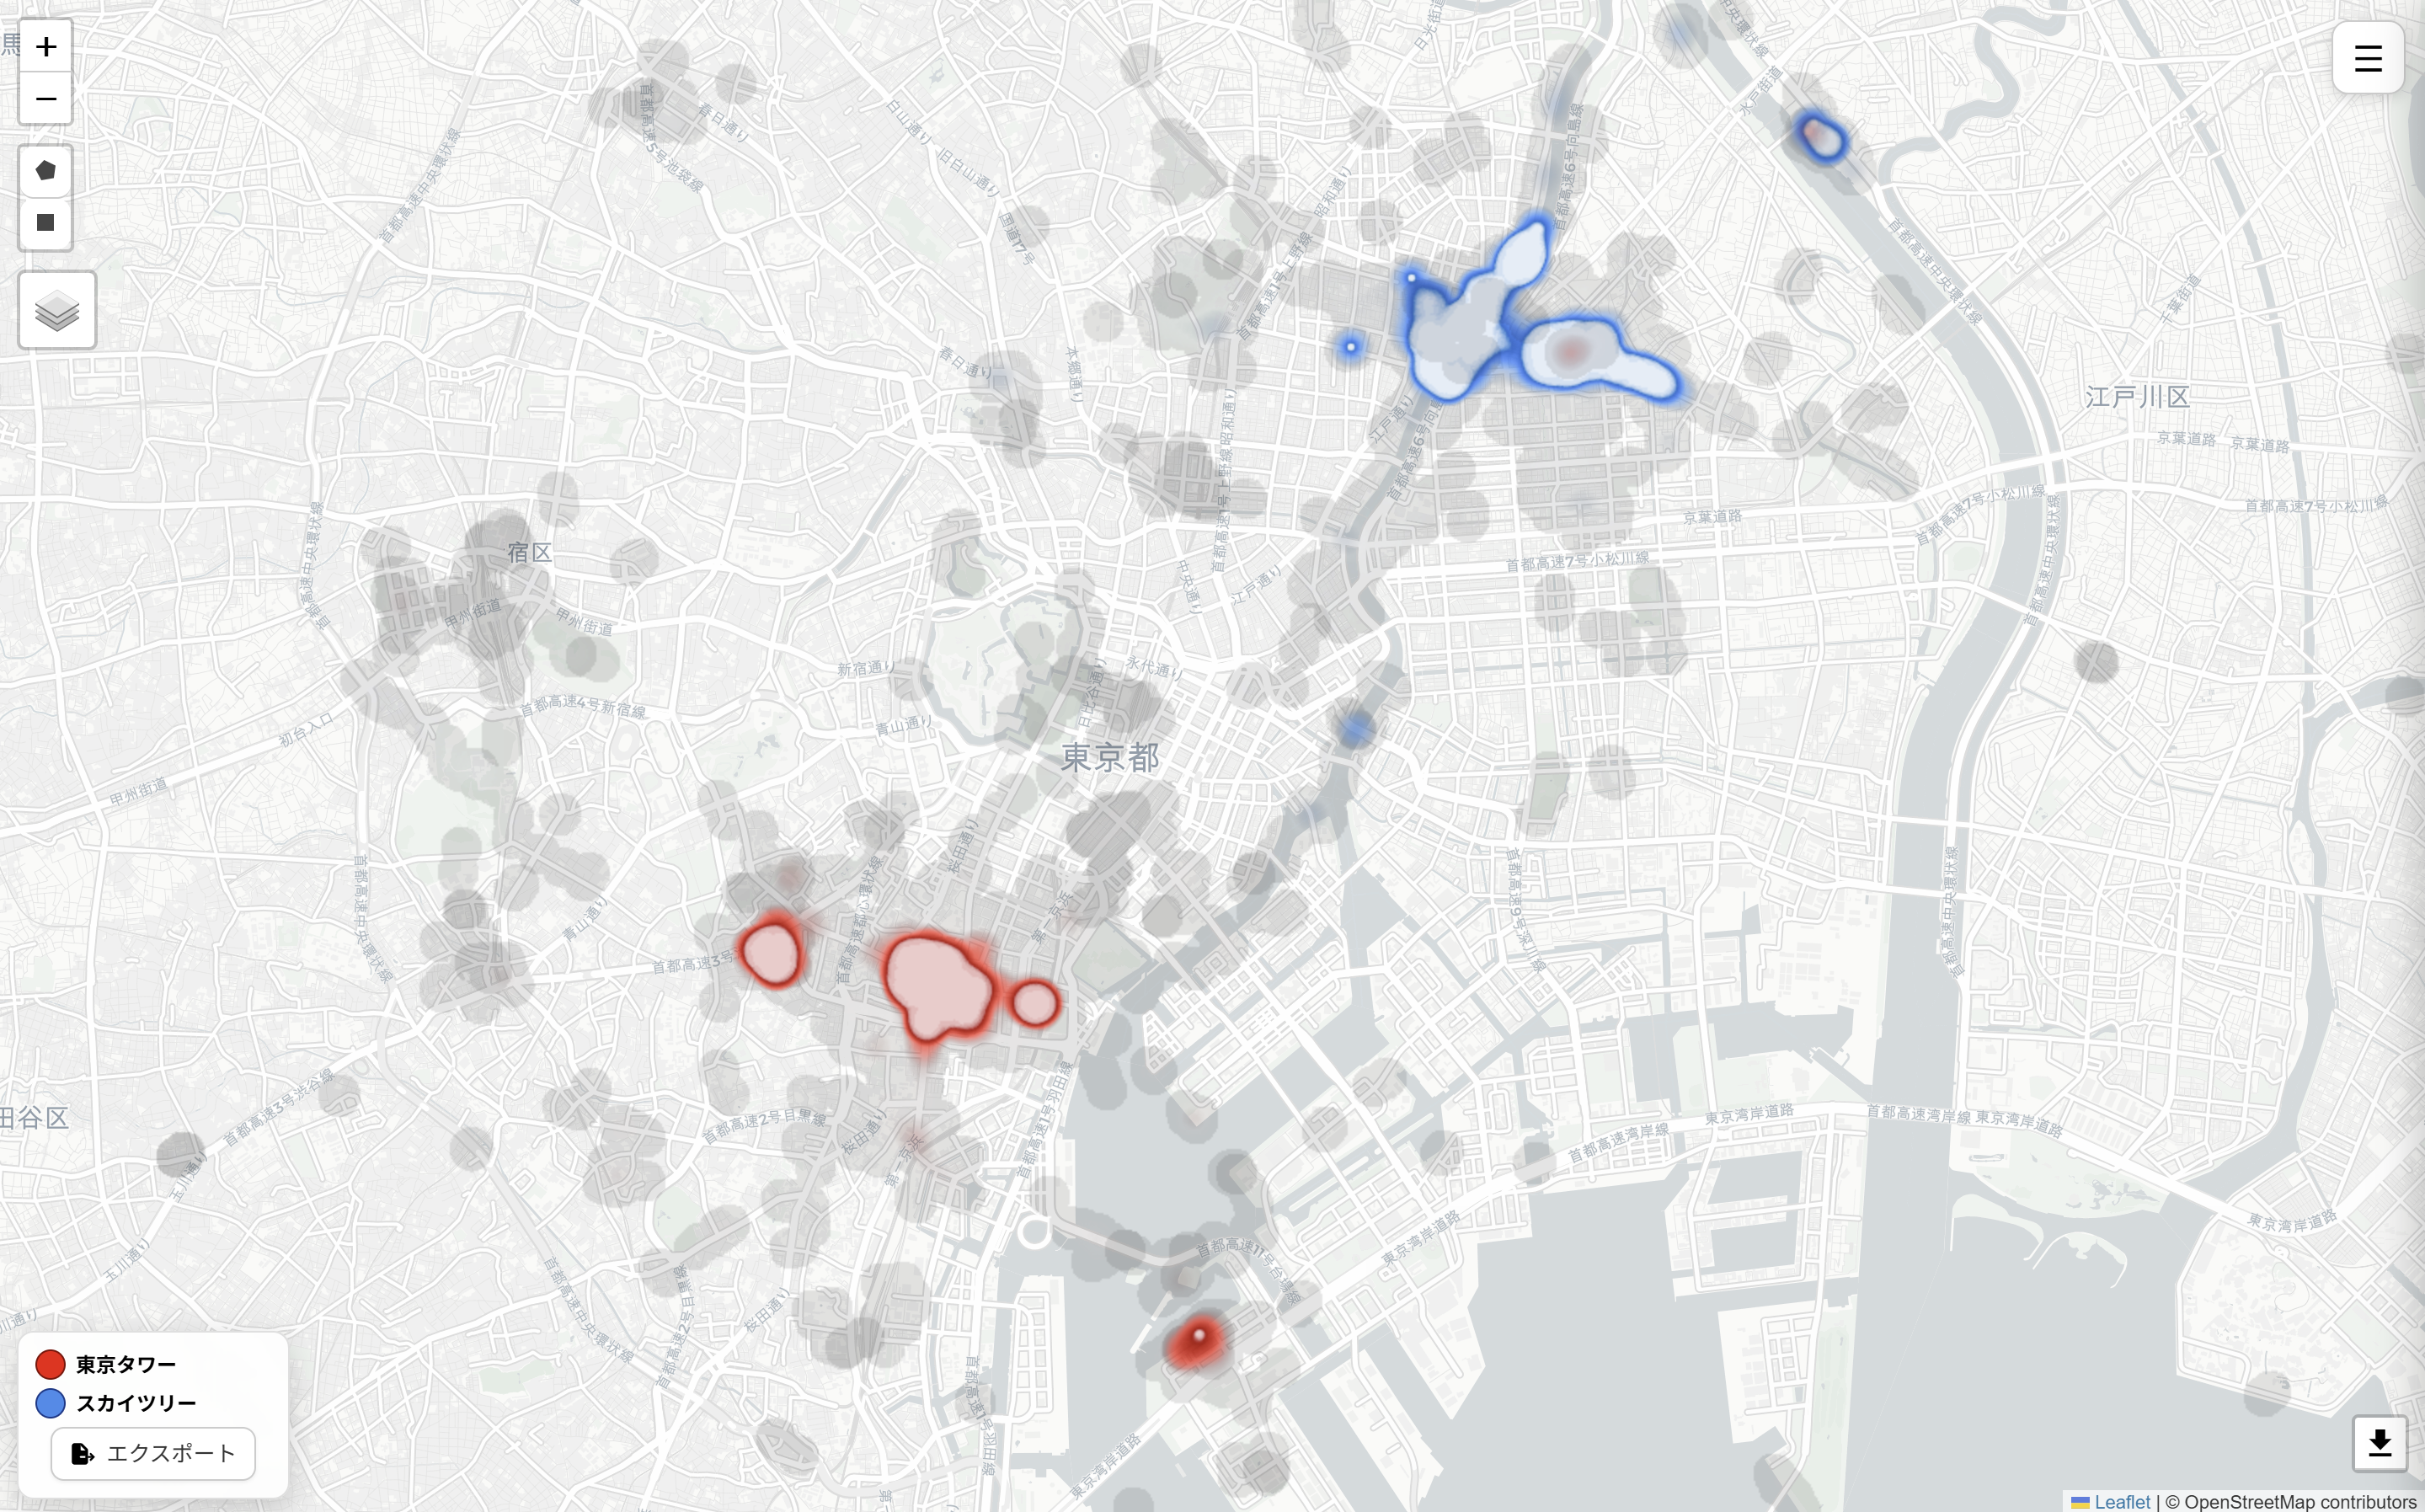
\includegraphics[width=0.9\textwidth]{figures/result_tower_heat.png}
  \caption{東京タワーとスカイツリーの撮影位置分布の可視化例(heatmap版)}
  \label{fig:tower_heatmap} 
\end{figure}

この図に表れているように、東京タワー近辺、スカイツリー近辺ではヒートマップが濃く描画されており、分布が集中している様子が視覚的に把握できる.また、両ランドマークから離れた地域ではヒートマップが薄くなっており、分布が疎である様子が視覚的に把握できる.

この例示に利用したコマンドを以下に示す.なお、APIKEYは各自で取得したものに置き換える必要がある.
\begin{commandline} 
npx -y -p splatone@latest crawler -p flickr \
-k "東京タワー#FA0000=tokyotower,東京タワー|スカイツリー#2B89EE=skytree,スカイツリー"  \
--vis-heat --v-heat-Radius=250 --p-flickr-APIKEY="aaaaaaaaaaaaaaaaaaaaaaaaaaaaaaaaaaaaaaaaa"
\end{commandline}

Heatmap Visualizationは描画を調整するために表\ref{tab:heat_params}に示すコマンドライン引数を受け取る.

\begin{table}[h]
\centering\small
\caption{Heatmap Visualizationの主なコマンドライン引数}
\label{tab:heat_params}
\begin{tabular}{llll}
\hline
引数 & 型 & 説明 & デフォルト \\
\hline
  \texttt{--vis-heat} & 真偽 & Heatmap Visualizationを有効にする & false \\
  \texttt{--v-heat-Radius} & 数値 & ヒートマップブラーの半径(Unitsで指定した距離単位) & 50 \\
  \texttt{--v-heat-Units} & 文字列 & Radiusに使用する距離単位(kilometers/meters/miles) & meters \\
  \texttt{--v-heat-MinOpacity} & 数値 & ヒートマップの最小透明度 & 0 \\
  \texttt{--v-heat-MaxOpacity} & 数値 & ヒートマップの最大透明度 & 1 \\
  \texttt{--v-heat-MaxValue} & 数値 & ヒートマップ強度の最大値(未指定時は自動推定) & (未指定) \\
  \texttt{--v-heat-WeightThreshold} & 数値 & 近傍点数がこの値未満の点は描画しない & 1 \\
\hline
\end{tabular}
\end{table}

\subsubsection{DBSCAN-based Visualization}

DBSCAN\cite{ester1996dbscan}は密度に基づくクラスタリング手法であり,特にノイズを含む空間データのクラスタリングに適している.DBSCANは,ユーザが指定した距離パラメータEpsと最小点数パラメータMinPtsに基づき,非線形なデータのまとまりを検出できる.具体的には,ある点の近傍にEps以内の点がMinPts以上存在する場合,その点はコア点として識別され,コア点同士が連結されることでクラスタが形成される.この特徴はジオソーシャルデータの分析と可視化に有用であり,多くの研究で採用されている\cite{shirai2013aoi,huang2015geographical,li2018spatial,zhang2020density}.

DBSCAN Visualizationでは,各クラスタをDBSCANにより空間クラスタリングし,結果を地図上に表示する.ここでの問題は、複数のカテゴリが混在し、かつ各カテゴリにおいて複数のクラスタが形成される場合である.この場合、各クラスタを個別色として描画すると,クラスタ数が多い場合、視覚的に煩雑になり、カテゴリとクラスタの理解が困難になる。クラスタの境界が複雑になるため,地図上での解釈が難しくなる.

この問題の根本的な解決は今後の課題であるが、現状においては、各クラスタのラベルに対して、そのクラスタに属する点から引き出し線を描画している。ラベルは任意の場所に移動・配置できるため、クラスタの境界が複雑であっても、ラベルを見やすい位置に配置することで、クラスタとカテゴリの関係を把握しやすくしている。

図~\ref{fig:tower_dbscan}に,東京タワーとスカイツリーの撮影位置分布をDBSCAN可視化で表現した例を示す.
\begin{figure}[h] 
  \centering
  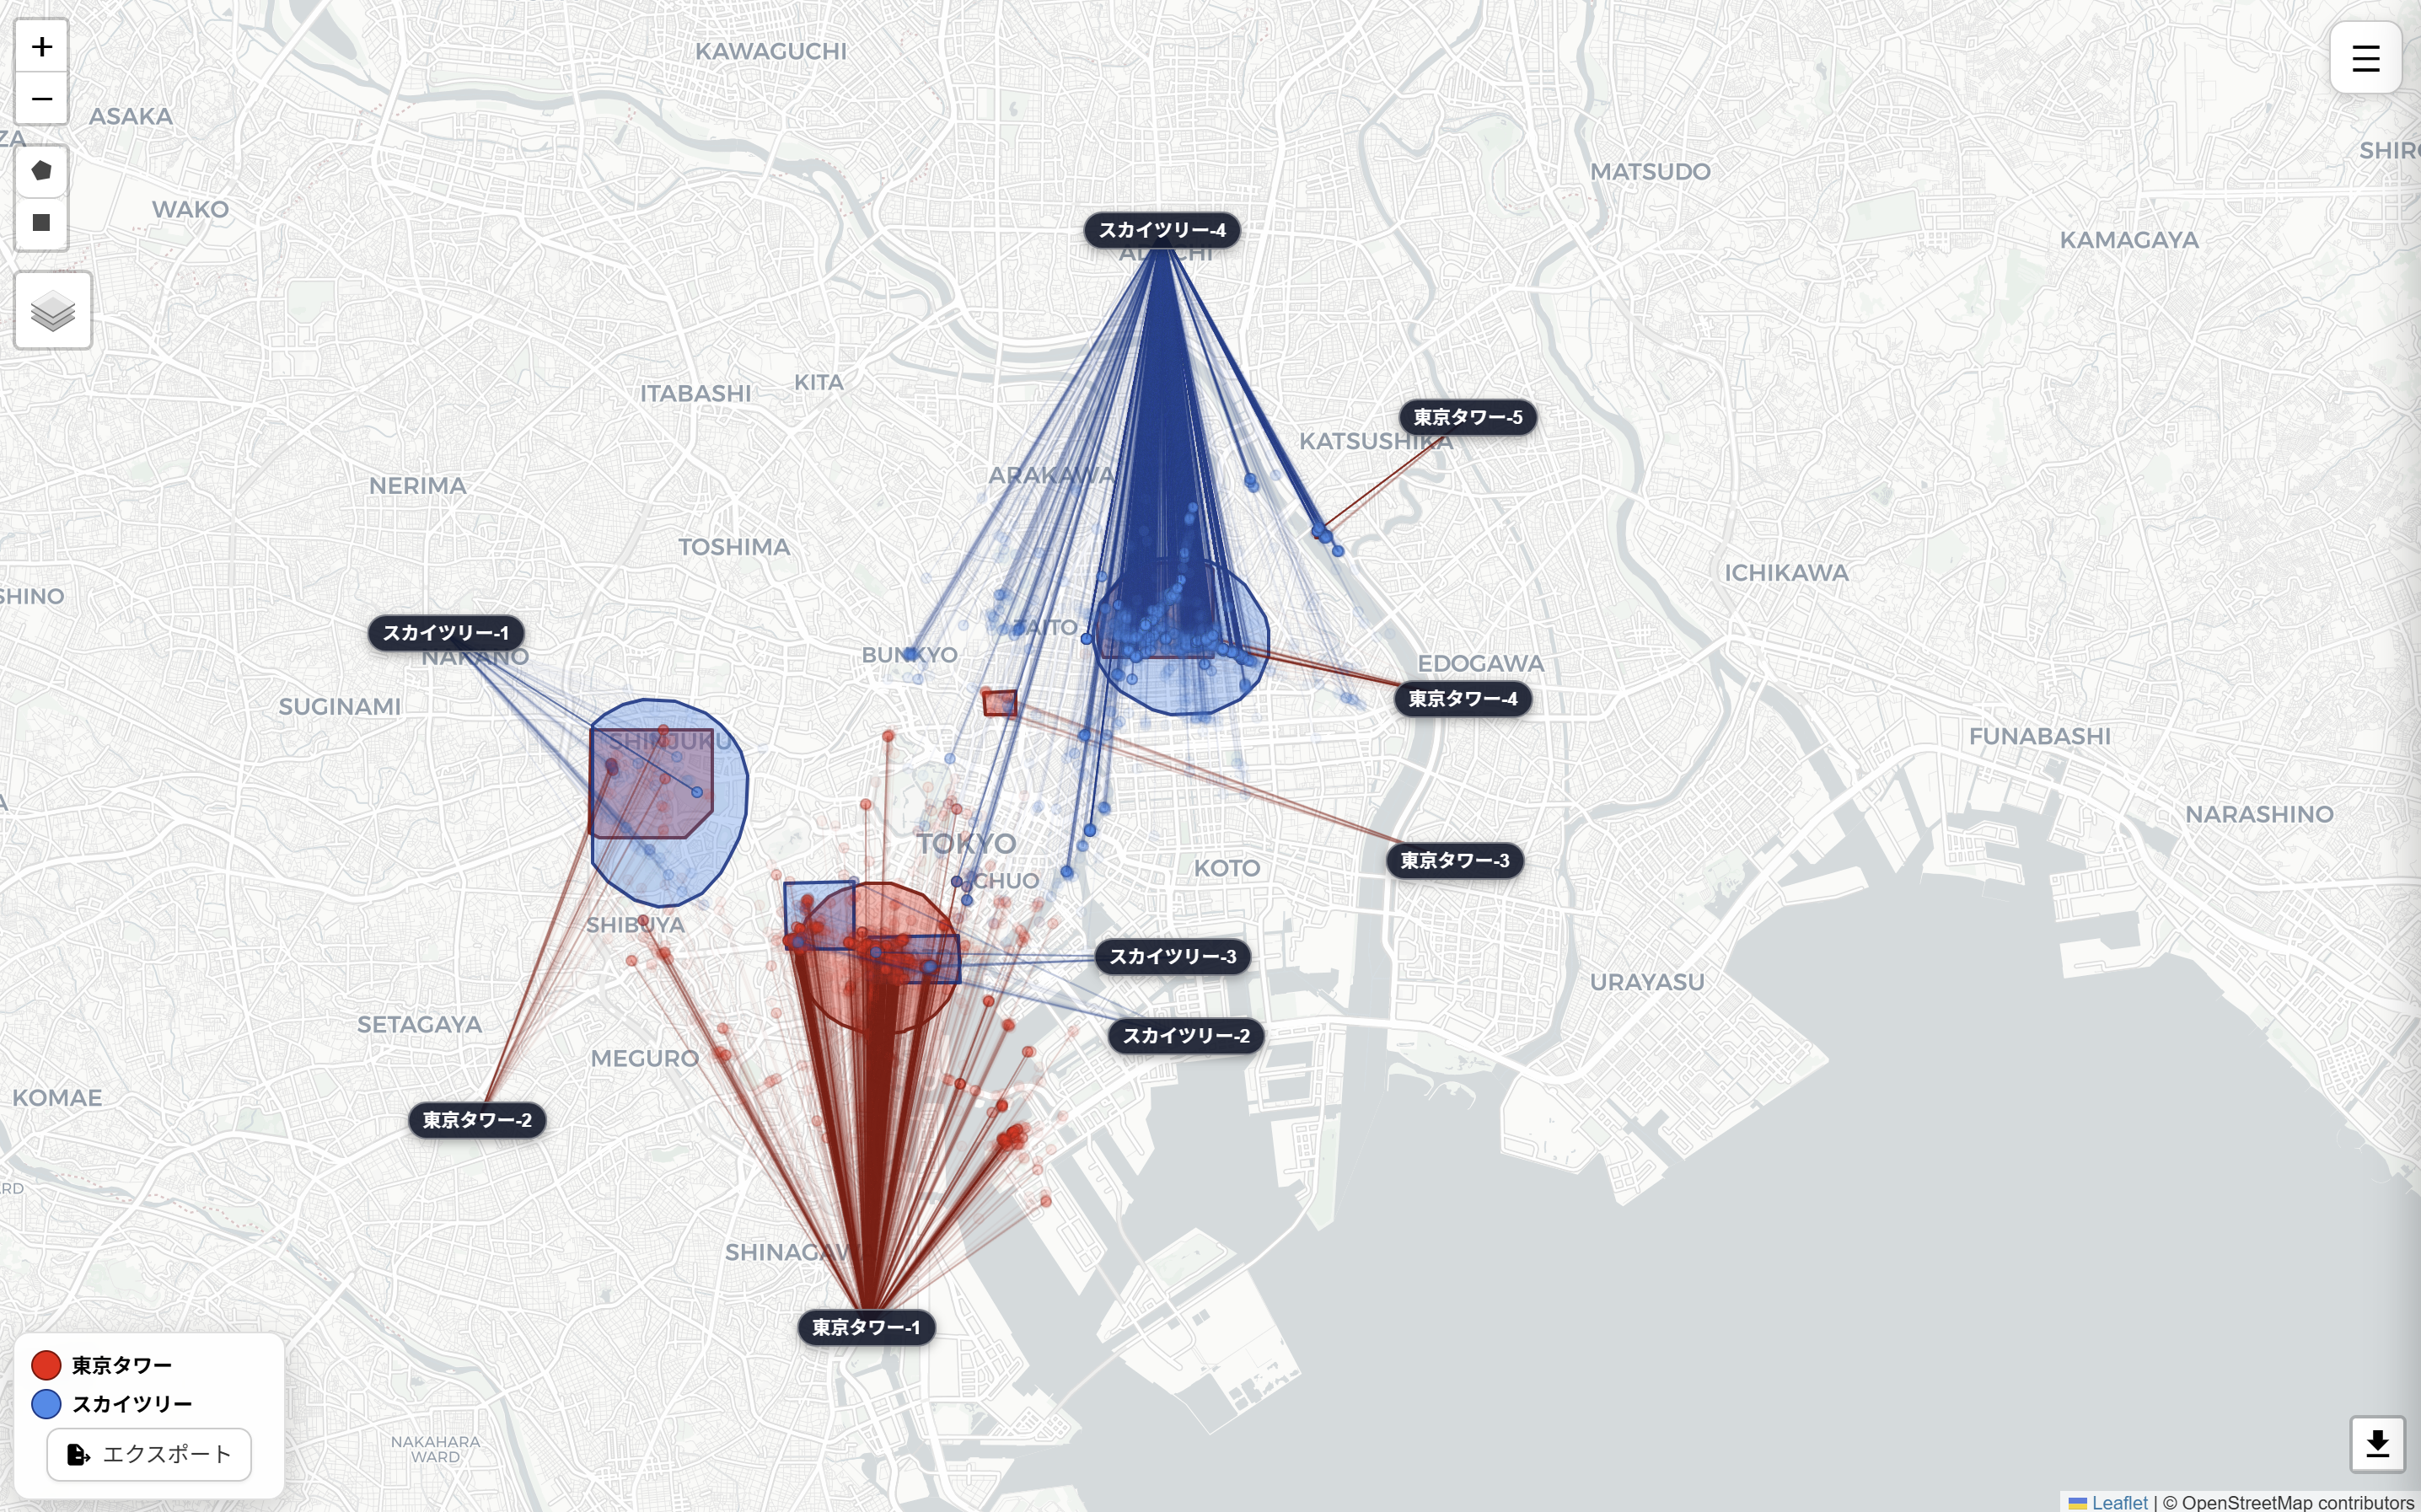
\includegraphics[width=0.9\textwidth]{figures/result_tower_dbscan.png}
  \caption{東京タワーとスカイツリーの撮影位置分布の可視化例(DBSCAN版)}
  \label{fig:tower_dbscan}
\end{figure}

この図に表れているように、東京タワー近辺とスカイツリー近辺に大きなクラスタが形成されており、加えて、有名な写真スポットにもクラスタが存在する事が視覚的に確認できる。

この例示に利用したコマンドを以下に示す.なお、APIKEYは各自で取得したものに置き換える必要がある.
\begin{commandline}
npx -y -p splatone@latest crawler -p flickr \
-k "東京タワー#FA0000=tokyotower,東京タワー|スカイツリー#2B89EE=skytree,スカイツリー"  \
--vis-dbscan --v-dbscan-MinPts=30 --v-dbscan-Eps=1 \
--p-flickr-APIKEY="aaaaaaaaaaaaaaaaaaaaaaaaaaaaaaaaaaaaaaaaaaaaaaa"
\end{commandline}

DBSCAN Visualizationは描画を調整するために表\ref{tab:dbscan_params}に示すコマンドライン引数を受け取る.

\begin{table}[h]
\centering\small
\caption{DBSCAN Visualizationの主なコマンドライン引数}
\label{tab:dbscan_params}
\begin{tabular}{llll}
\hline
引数 & 型 & 説明 & デフォルト \\
\hline
  \texttt{--vis-dbscan} & 真偽 & DBSCAN Visualizationを有効にする & false \\
  \texttt{--v-dbscan-Eps} & 数値 & DBSCANのeps(クラスタ判定距離) & 0.6 \\
  \texttt{--v-dbscan-MinPts} & 数値 & クラスタ確定に必要な点数 & 6 \\
  \texttt{--v-dbscan-Units} & 文字列 & epsの距離単位(kilometers/meters/miles) & kilometers \\
  \texttt{--v-dbscan-StrokeWidth} & 数値 & ポリゴン輪郭の太さ & 2 \\
  \texttt{--v-dbscan-StrokeOpacity} & 数値 & ポリゴン輪郭の透明度 & 0.9 \\
  \texttt{--v-dbscan-FillOpacity} & 数値 & ポリゴン塗りの透明度 & 0.35 \\
  \texttt{--v-dbscan-DashArray} & 文字列 & LeafletのdashArray指定(例: "4 6") & (空文字) \\
  \texttt{--v-dbscan-KernelScale} & 数値 & KDEカーネル半径をepsの何倍にするか & 1 \\
  \texttt{--v-dbscan-GridSize} & 数値 & KDE計算用グリッド解像度(長辺方向セル数) & 80 \\
  \texttt{--v-dbscan-ContourPercent} & 数値 & 最大密度に対する等値線レベル(0-1) & 0.4 \\
\hline
\end{tabular}
\end{table}


\section{Implementation}
\label{sec:implementation}
Splatone CrawlerはNode.jsをベースとしたツールチェインとして実装されており,画像収集を行うCrawler,カラーパレット生成や空間集計を行うライブラリ群,および可視化結果を提示するWeb UIから構成される.
ライブラリコードは主に `lib/` 以下に配置されており,`splatone.js` はコマンドラインツールとして各種処理を統合するエントリポイントの役割を担う.

Provider拡張機構は,`lib/ProviderBase.js`と`lib/providerLoader.js`により提供される.
各Visualizerやデータソースは,この基底クラスを継承して必要なメソッドを実装することで,Splatone Crawler本体から一貫した方法で呼び出せるようになっている.
これにより,新しいデータソースや可視化手法を追加する際にも,既存のコードに対する修正を最小限に抑えつつ拡張が可能である.

Web UIは`public/`および`views/`以下に実装されており,サーバ側はNode.jsのHTTPサーバとテンプレートエンジンを用いている.
ユーザはブラウザ上でVisualizerを切り替えたり,クラスタリングパラメータを調整したりしながら,画像コレクションの空間的・色彩的特徴を対話的に探索できる.

\subsection{Web UI}
\label{sec:webui}

\subsection{Result Browse Mode}
\label{sec:resultbrowse}

\subsection{Provider Extension Mechanism}
\label{sec:providerextension}
\subsection{Visualization Extension Mechanism}
\label{sec:visualizationextension}


\section{Use Cases}
\label{sec:usecases}
% 例: Flickr 画像を用いた都市・景観の色分布解析など

\section{Discussion}
\label{sec:discussion}
% 利点・限界・今後の展望

\subsection{マルチレイヤ可視化の限界}
% レイヤの順序問題を書き、それを解決する新たな可視化手法の必要性を議論

\subsection{複数のProviderの統合的利用に関する議論}
% 現在はProviderはFlickrに限定されているが、将来的には複数のProviderを実装予定である。現在のアーキテクチャではProviderは一つしか指定できないようになっている
% 複数に拡張するには、Provider間でデータを統合する仕組みが必要となる。これは実装上の問題点というよりは、例えばFlickrとInstagramのような同種のProvider間でのデータ統合と、FlickrとOpen StreetMapのような異種のProvider間でのデータ統合とで、異なる統合方法を取る必要があるかもしれない。
% この点を特定のProviderに依存しないSplatone Crawlerの特徴を活かしつつ、どのように実現するかが今後の課題である。


\section{Conclusion}
\label{sec:conclusion}
% 本ツールのまとめと今後の課題

%\section*{Acknowledgements}
% 謝辞があれば記載

\bibliographystyle{plain}
\bibliography{references}

\end{document}
